%----------------------------------------------------------------------------------------
%	PACKAGES AND OTHER DOCUMENT CONFIGURATIONS
%----------------------------------------------------------------------------------------

\documentclass{article}

\usepackage{fancyhdr} % Required for custom headers
\usepackage{lastpage} % Required to determine the last page for the footer
\usepackage{extramarks} % Required for headers and footers
\usepackage{graphicx} % Required to insert images
\usepackage{pdflscape} % Allow us to make certain pages in landscape orientation
\usepackage{amsmath} % Allow multiple line equations
\usepackage{amssymb}
\usepackage{scrextend}
\usepackage{xcolor}
\usepackage{listings}

\definecolor{mGreen}{rgb}{0,0.6,0}
\definecolor{mGray}{rgb}{0.5,0.5,0.5}
\definecolor{mPurple}{rgb}{0.58,0,0.82}
\definecolor{backgroundColour}{rgb}{0.95,0.95,0.92}

\lstdefinestyle{CStyle}{
    backgroundcolor=\color{backgroundColour},   
    commentstyle=\color{mGreen},
    keywordstyle=\color{magenta},
    numberstyle=\tiny\color{mGray},
    stringstyle=\color{mPurple},
    basicstyle=\footnotesize,
    breakatwhitespace=false,         
    breaklines=true,                 
    captionpos=b,                    
    keepspaces=true,                 
    numbers=none,                   
    numbersep=5pt,                  
    showspaces=false,                
    showstringspaces=false,
    showtabs=false,                  
    tabsize=2,
    language=C
}

% Margins
\topmargin=-0.45in
\evensidemargin=0in
\oddsidemargin=0in
\textwidth=6.5in
\textheight=9.0in
\headsep=0.25in 

\linespread{1.1} % Line spacing

% Set up the header and footer
\pagestyle{fancy}
\chead{\Title} % Top center header
\rhead{\firstxmark} % Top right header
\lfoot{\lastxmark} % Bottom left footer
\cfoot{} % Bottom center footer
\rfoot{Page\ \thepage\ of\ \pageref{LastPage}} % Bottom right footer
\renewcommand\headrulewidth{0.4pt} % Size of the header rule
\renewcommand\footrulewidth{0.4pt} % Size of the footer rule

\setlength\parindent{0pt} % Removes all indentation from paragraphs

%----------------------------------------------------------------------------------------
%	DOCUMENT STRUCTURE COMMANDS
%----------------------------------------------------------------------------------------

\setcounter{secnumdepth}{0} % Removes default section numbers
   
%----------------------------------------------------------------------------------------
%	NAME AND CLASS SECTION
%----------------------------------------------------------------------------------------

\newcommand{\Title}{Assignment 1} % Assignment title
\newcommand{\DueDate}{21 April 2018} % Due date
\newcommand{\Class}{CAB202 - Microprocessors and Digital Systems} % Course/class
\newcommand{\AuthorName}{Pedro Alves (n9424342)}

%----------------------------------------------------------------------------------------
%	TITLE PAGE
%----------------------------------------------------------------------------------------

\title{
\vspace{2in}
\textmd{\huge\textbf{\Class}}\\
\textmd{{\Title}}\\
\vspace{3in}
\textmd{{\AuthorName}}\\
}

%----------------------------------------------------------------------------------------

\begin{document}

\maketitle
\clearpage

%----------------------------------------------------------------------------------------
%	TABLE OF CONTENTS
%----------------------------------------------------------------------------------------

%\setcounter{tocdepth}{1} % Uncomment this line if you don't want subsections listed in the ToC

\newpage
\tableofcontents
\newpage

%----------------------------------------------------------------------------------------
%	EXECUTIVE SUMMARY
%----------------------------------------------------------------------------------------
\section{Executive Summary}
The obejctive of this report is to give a brief explanation of how the game \emph{Race to Zombie Mountain} was implemented. It also includes multiple tests that serve to verify the claims made in this report. 
\newline
A score and highscore table system were developed as an extension to the basic game. The highscore table can hold information about the score and the name of the player for the top 100 scores. This data is held on a local file called \emph{highscores}. 
\clearpage

%----------------------------------------------------------------------------------------
%	SPLASH SCREEN
%----------------------------------------------------------------------------------------
\section{Splash Screen}
 The splash screen is the first screen the player sees when they start the game. It provides basic information about the game and will change to the main game screen when the player presses any key.

\subsection*{Functions}
\begin{lstlisting}[style=CStyle]
	// main.c
	void update_start_screen();
\end{lstlisting}
Called every tick of the main game loop. Will change the game's state to \emph{GAME\_SCREEN} if there is any key in the input buffer. Since the \emph{change\_state()} function already purges the input buffer, we do not have to worry about the game skipping straight to the \emph{GAME\_SCREEN}.
\begin{lstlisting}[style=CStyle]
	// main.c
	void draw_start_screen();
\end{lstlisting}
Calculates the x and y coordinates of each string to be shown based on the dimensions of the screen. Will then call \emph{draw\_string()} and \emph{draw\_center\_text()} multiple times to add the strings to the desired location.
\begin{lstlisting}[style=CStyle]
	// main.c
	void draw_center_text(char * text, int y);
\end{lstlisting}
Calculates what x coordinate is required in order to have the text appear at the middle of the screen. Then calls \emph{draw\_string()} to print the text. 
\newline

\subsection*{Testing}
Testing that the splash screen shows up when the game is started.
\begin{figure}[h]
	\begin{center}
	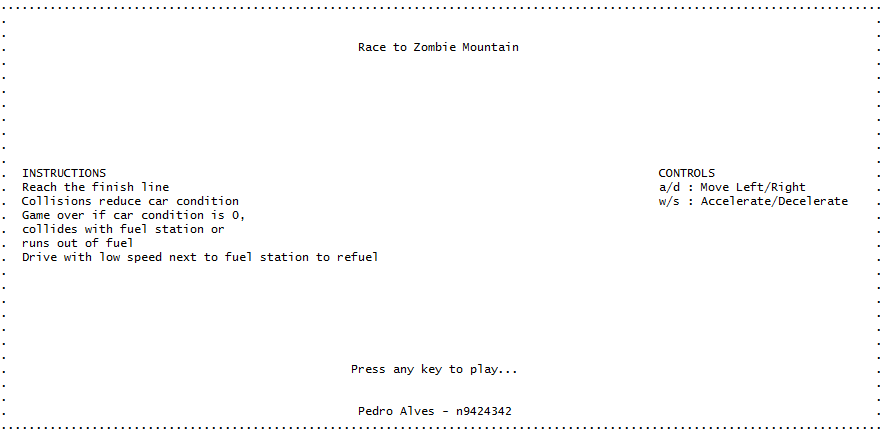
\includegraphics[width=1\textwidth]{images/splash_screen}
	\caption{The splash screen when the player starts the game}
	\label{fig:splash_screen} 
	\end{center}
\end{figure}

\clearpage

%----------------------------------------------------------------------------------------
%	BORDER
%----------------------------------------------------------------------------------------
\section{Border}
The border is simply a rectangle that is drawn on the edge of the terminal. It supports every terminal size.
\newline
The \emph{draw\_borders()} functon is the last one called before \emph{show\_screen()} in the draw step of the game loop. This ensures that no other graphics ever block the border. 

\subsection*{Globals}
\begin{lstlisting}[style=CStyle]
	// zombiemountain.h
	#define BORDER_CHAR	46
\end{lstlisting}
The character that will be used to represent the border. The number 46 represents the ASCII character "." (full stop).
\newline

\subsection*{Functions}
\begin{lstlisting}[style=CStyle]
	// main.c
	void draw_borders();
\end{lstlisting}
Draws 4 lines that form a rectangle on the edge of the screen. The length of these lines are calculated by using the screen width and height in order to make the borders work on every screen size.
\newline

\subsection*{Testing}
The game is started in different sized terminals and the borders are verified to have been drawn correctly.
\subsubsection*{Screen: 80x24}
\begin{figure}[h]
	\begin{center}
	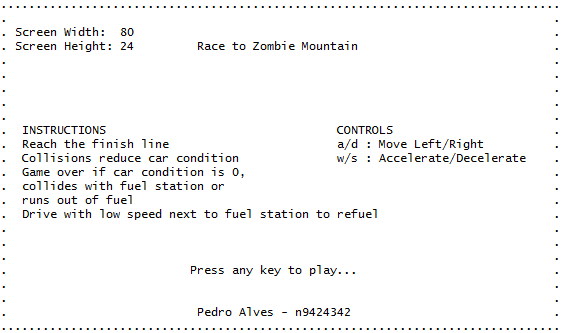
\includegraphics[width=0.95\textwidth]{images/border_80x24}
	\caption{The border with screen dimensions of 80x24}
	\label{fig:border_80x24} 
	\end{center}
\end{figure}
\subsubsection*{Screen: 126x31}
\begin{figure}[h]
	\begin{center}
	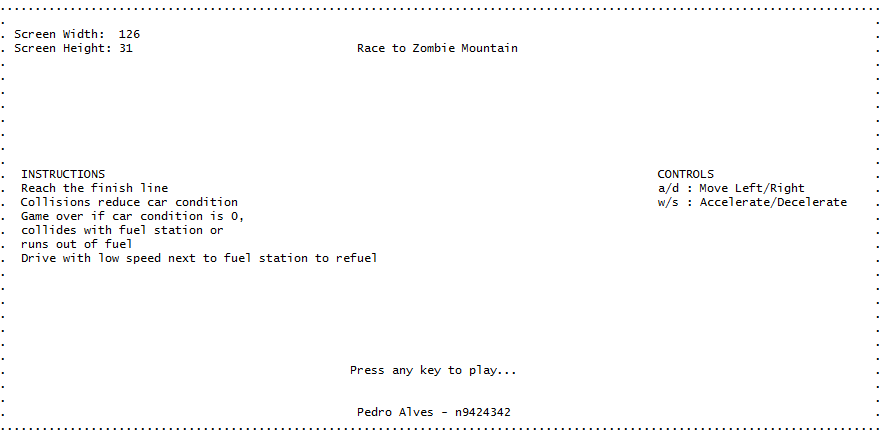
\includegraphics[width=1\textwidth]{images/border_126x31}
	\caption{The border with screen dimensions of 126x31}
	\label{fig:border_126x31} 
	\end{center}
\end{figure}
\subsubsection*{Screen: 190x50}
\begin{figure}[!ht]
	\begin{center}
	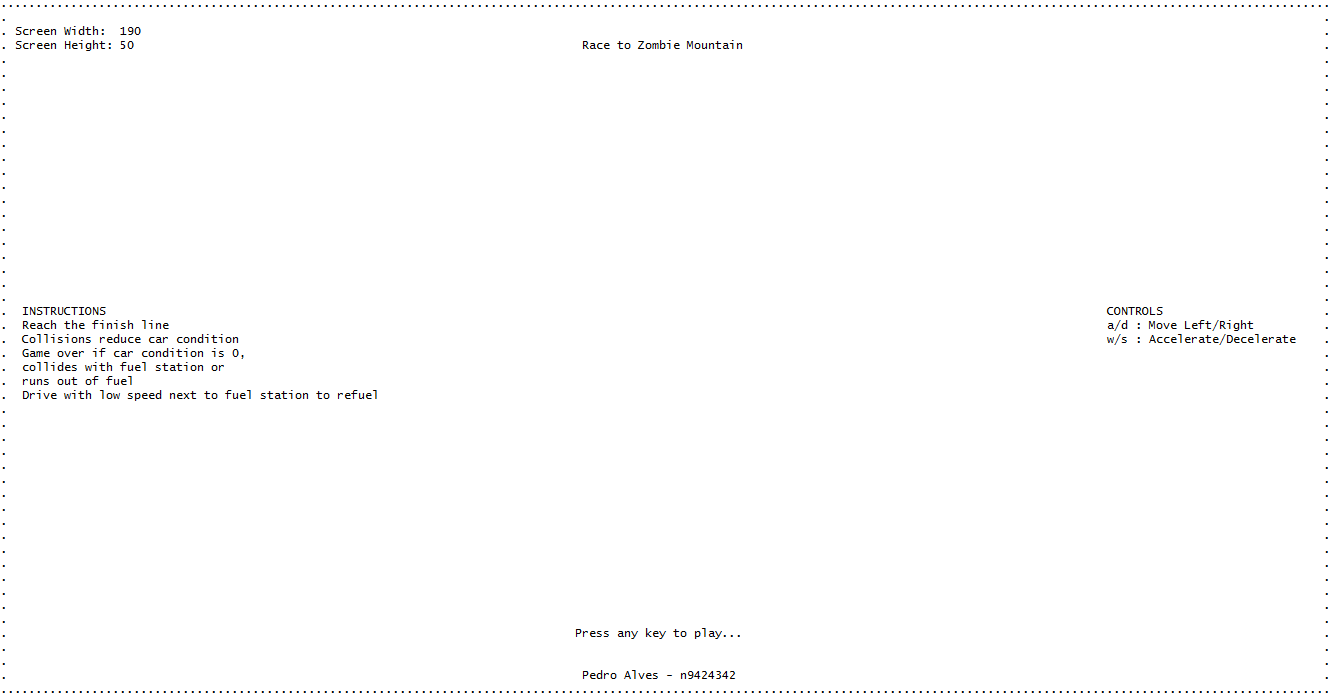
\includegraphics[width=0.77\paperwidth]{images/border_190x50}
	\caption{The border with screen dimensions of 190x50}
	\label{fig:border_190x50} 
	\end{center}
\end{figure}

\clearpage
%----------------------------------------------------------------------------------------
%	DASHBOARD
%----------------------------------------------------------------------------------------
\section{Dashboard}
A sub-window in the terminal which displays data regarding the player's car such as condition, speed and fuel as well as displaying stats on the game itself such as time spent and total distance travelled. 
\newline
Warnings also appear on the dashboard to notify the player that the car is offroad or is refuelling.

\subsection*{Globals}
\begin{lstlisting}[style=CStyle]
	// zombiemountain.h
	int dashboard_x;
\end{lstlisting}
The x-coordinate of the border between the dashboard and the playing area.
\begin{lstlisting}[style=CStyle]
	// obstacles.h
	#define DASHBOARD_SIZE	20
\end{lstlisting}
The width of the dashboard.
\begin{lstlisting}[style=CStyle]
	// zombiemountain.h
	#define DASHBOARD_BORDER_CHAR	47
\end{lstlisting}
The ASCII character that will represent the border that separates the playing area and the dashboard.
\begin{lstlisting}[style=CStyle]
	// zombiemountain.h
	int speed;
\end{lstlisting}
The current speed of the player.
\begin{lstlisting}[style=CStyle]
	// zombiemountain.h
	int fuel;
\end{lstlisting}
The current fuel available to the player.
\begin{lstlisting}[style=CStyle]
	// obstacles.h
	int car_condition;
\end{lstlisting}
The condition of the car as a percentage.
\begin{lstlisting}[style=CStyle]
	// hscore.h
	int score;
\end{lstlisting}
The current score of the player.
\begin{lstlisting}[style=CStyle]
	// zombiemountain.h
	int distance_travelled;
\end{lstlisting}
The distance travelled since the start of the game.
\begin{lstlisting}[style=CStyle]
	// zombiemountain.h
	double game_start_time;
\end{lstlisting}
The time in milliseconds that the game started.
\begin{lstlisting}[style=CStyle]
	// zombiemountain.h
	timer_id refuel_timer;
\end{lstlisting}
A timer that is set when the car starts refuelling.
\newline

\subsection*{Functions}
\begin{lstlisting}[style=CStyle]
	// main.c
	void draw_dashboard();
\end{lstlisting}
Draws a border between the playing area and the dashboard area. Calls \emph{draw\_string()} and \emph{draw\_int()} multiple times to print the relevant globals and their captions.
\newline
If the car is offroad or refuelling, a relevant warning will also be drawn. Additionaly for refuelling, will display how long until it is finished.
\newline
\begin{lstlisting}[style=CStyle]
	// main.c
	bool car_offroad();
\end{lstlisting}
Checks if any portion of the car is outside the road boundaries and return true if so.
\begin{lstlisting}[style=CStyle]
	// main.c
	double refuel_time_left();
\end{lstlisting}
Calculates how much time is left to finish refuelling. This is done by calculating the difference between the current time and the time the \emph{refuel\_timer} is meant to reset, this is then subtracted from \emph{3.0}.
\newline

\subsection*{Testing}
\subsubsection*{Stats are modified with gameplay}
Two screenshots of the same gameplay are taken where the fuel is checked if it is decreased and the time,distance and score are increased.
\begin{figure}[!ht]
	\begin{center}
	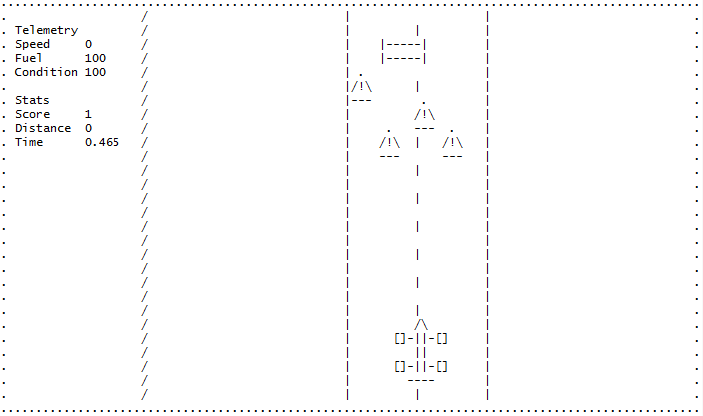
\includegraphics[width=0.75\paperwidth]{images/dashboard_test_statschange}
	\caption{A screenshot of the game as it starts}
	\label{fig:dashboard_test_stats} 
	\end{center}
\end{figure}
\newline
Figure \ref{fig:dashboard_test_stats} shows the dashboard on the left side of the terminal with a border clearly separating it from the playing area. To achieve the second part of the test, the 'w' key was pressed 3 times to test if the speed is increased and the car was moved horizontally where necessary to avoid obstacles. 
\newline
The condition stat will be tested in the \emph{Collision} section and the refuelling warning and timer will be tested in the \emph{Fuel} section.  
\newpage
\begin{figure}[!ht]
	\begin{center}
	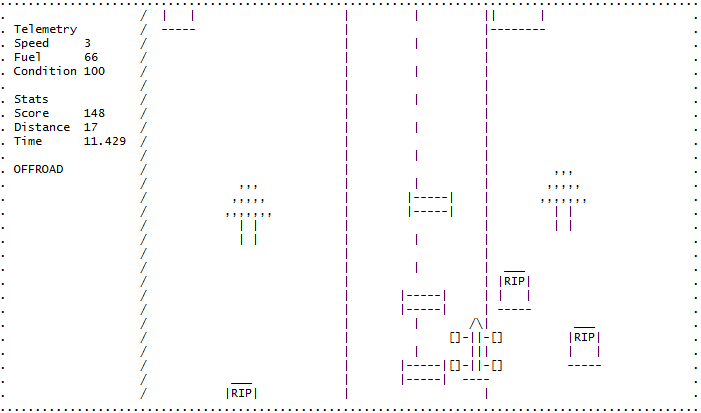
\includegraphics[width=0.75\paperwidth]{images/dashboard_test_statschange2}
	\caption{A screenshot of the same game sessions as the figure above but 11 seconds into gameplay}
	\label{fig:dashboard_test_stats2} 
	\end{center}
\end{figure}
Figures \ref{fig:dashboard_test_stats} and \ref{fig:dashboard_test_stats2} show that the stats are represented in the dashboard and change when supposed to. The \emph{OFFROAD} warning also appears when the car moves beyond the border of the road. 
\newline
Figure \ref{fig:dashboard_test_fuelwarning} shows the low fuel warning appears when fuel falls below 25\%.
\begin{figure}[!ht]
	\begin{center}
	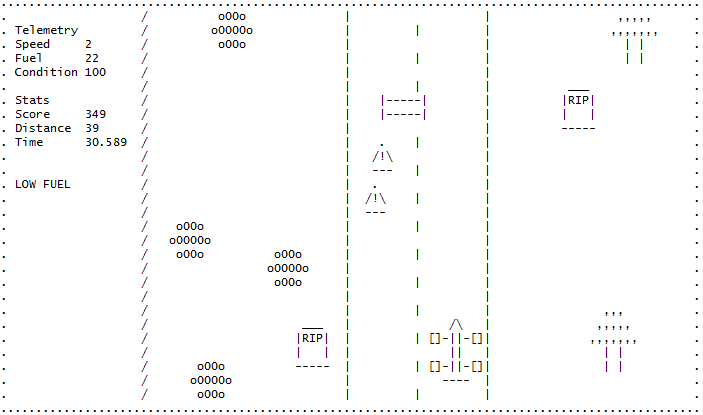
\includegraphics[width=0.667\paperwidth]{images/dashboard_test_fuelwarning}
	\caption{Low Fuel warning appearing when fuel is below 1/4 the maximum}
	\label{fig:dashboard_test_fuelwarning} 
	\end{center}
\end{figure}
\clearpage

%----------------------------------------------------------------------------------------
%	RACE CAR AND HORIZONTAL MOVEMENT
%----------------------------------------------------------------------------------------
\section{Race Car and Horizontal Movement}
The race car is a sprite 8 units wide and 5 units tall. This sprite is always stuck in the same position with the illusion of movement given by the obstacles being moved downwards. The speed at which the obstacles move is proportional to the speed setting.

\subsection*{Globals}
\begin{lstlisting}[style=CStyle]
	// imagemngr.h
	#define PLAYER_WIDTH	8
\end{lstlisting}
The width of the car sprite.
\begin{lstlisting}[style=CStyle]
	// imagemngr.h
	#define PLAYER_HEIGHT	5
\end{lstlisting}
The height of the car sprite
\begin{lstlisting}[style=CStyle]
	// zombiemountain.h
	#define INPUT_MOVE_LEFT		'a'
\end{lstlisting}
The keyboard input that will make the car turn left.
\begin{lstlisting}[style=CStyle]
	// zombiemountain.h
	#define INPUT_MOVE_RIGHT	'd'
\end{lstlisting}
The keyboard input that will make the car turn right
\begin{lstlisting}[style=CStyle]
	// zombiemountain.h
	sprite_id player;
\end{lstlisting}
The car sprite which the player controls.
\newline

\subsection*{Functions}
\begin{lstlisting}[style=CStyle]
	// main.c
	void setup_player_car();
\end{lstlisting}
Place the car sprite in the middle of the road, 2 units above the bottom of the screen. Also sets the car condition to 100\% and fuel to max.
\begin{lstlisting}[style=CStyle]
	// main.c
	void handle_input();
\end{lstlisting}
Get the next character from the input buffer. If it is a valid key, call the specific input handler. 
\begin{lstlisting}[style=CStyle]
	// main.c
	void handle_movement_input(int key);
\end{lstlisting}
Checks if the \emph{key} variable wants the car to turn left or right. Will then check if the car will be in the bounds of the playing area, if it'll collide laterally with any obstacle and if the speed is above zero. If all three checks pass, then the \emph{sprite\_move()} function is called.
\begin{lstlisting}[style=CStyle]
	// main.c
	bool in_bounds(int x, int y)
\end{lstlisting}
Checks if the \emph{(x,y)} coordinate is in bounds of the playing area, returns true if so.
\newline
\newpage

\subsection*{Testing}
\subsubsection*{Car doesn't move when speed is 0}
\begin{figure}[!ht]
	\begin{center}
	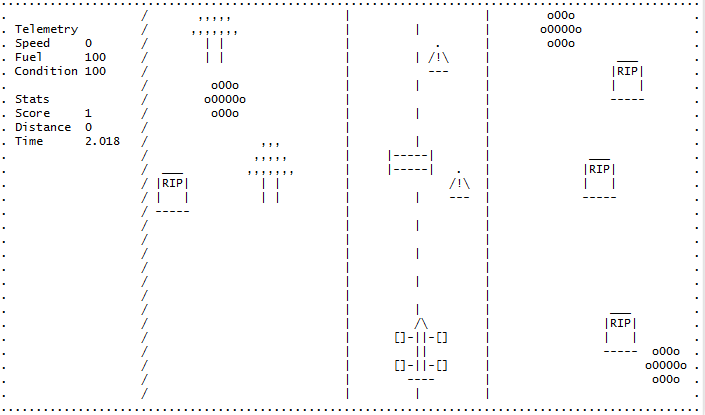
\includegraphics[width=0.667\paperwidth]{images/car_test_nospeed}
	\caption{Car in the middle of the road with speed equal zero}
	\label{fig:car_test_nospeed} 
	\end{center}
\end{figure}
The following inputs were pressed and the result shown in Figure \ref{fig:car_test_nospeed}: "a,d,a,d"
\begin{figure}[!ht]
	\begin{center}
	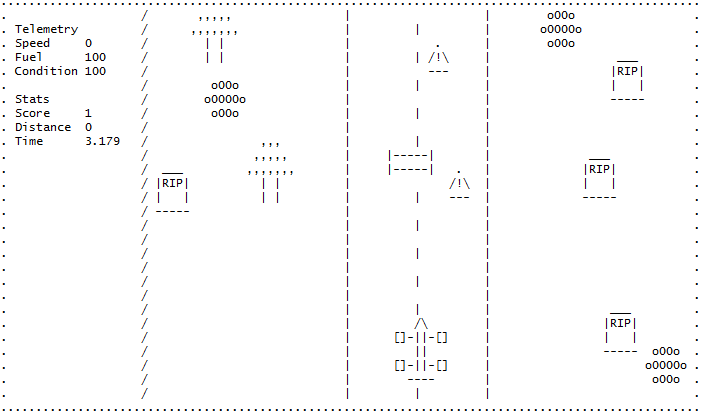
\includegraphics[width=0.667\paperwidth]{images/car_test_nospeed2}
	\caption{Results after attempting to move horizontally with speed equal zero}
	\label{fig:car_test_nospeed2} 
	\end{center}
\end{figure}

\subsubsection*{Car moves left and right}
From the position in Figure \ref{fig:car_test_nospeed2}, the following inputs were pressed "w,a,a,a".
\begin{figure}[!ht]
	\begin{center}
	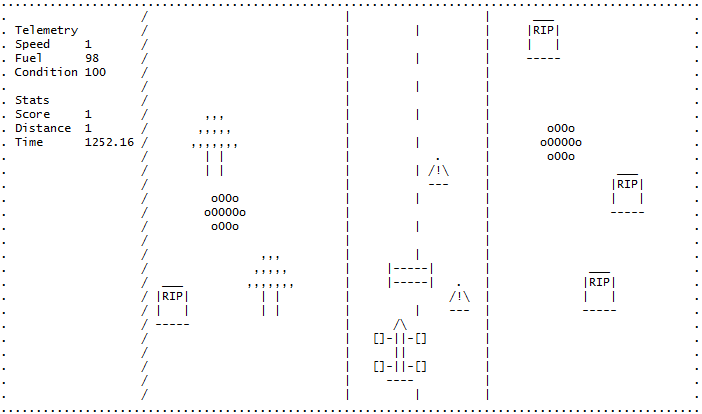
\includegraphics[width=0.667\paperwidth]{images/car_test_moveleft}
	\caption{Moving the car left with speed equal 1}
	\label{fig:car_test_moveleft} 
	\end{center}
\end{figure}
\newline
After the car is reset due to the inetivable collision in Figure \ref{fig:car_test_moveleft}, the following inputs were pressed "w,d,d,d". 
\begin{figure}[!ht]
	\begin{center}
	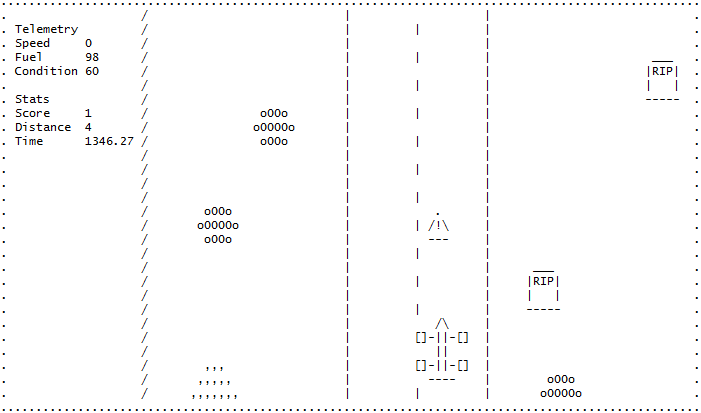
\includegraphics[width=0.667\paperwidth]{images/car_test_moveright}
	\caption{Moving the car right with speed equal 1 (car was stopped to grab screenshot)}
	\label{fig:car_test_moveright} 
	\end{center}
\end{figure}
\newpage

\subsubsection*{Car stays in bounds}
The car was moved to both extremes of the playing area with the lateral movement input held down. Figure \ref{fig:car_test_rightborder} shows the result of holding down 'd' and Figure \ref{fig:car_test_leftborder} shows the result of holding down 'a'.
\begin{figure}[!ht]
	\begin{center}
	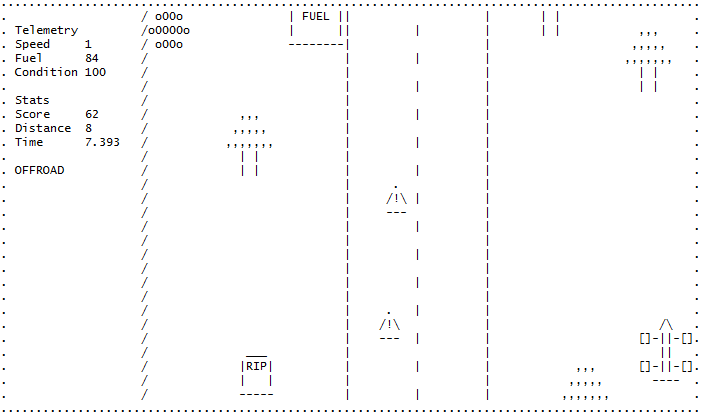
\includegraphics[width=0.667\paperwidth]{images/car_test_rightborder}
	\caption{Result of holding down 'd' when next to the right border}
	\label{fig:car_test_rightborder} 
	\end{center}
\end{figure}
\begin{figure}[!ht]
	\begin{center}
	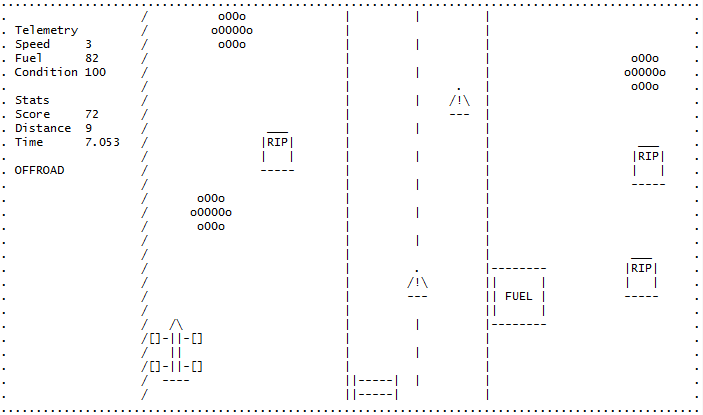
\includegraphics[width=0.667\paperwidth]{images/car_test_leftborder}
	\caption{Result of holding down 'a' when next to the left border}
	\label{fig:car_test_leftborder} 
	\end{center}
\end{figure}

\clearpage

%----------------------------------------------------------------------------------------
%	ACCELERATION AND SPEED
%----------------------------------------------------------------------------------------
\section{Acceleration and Speed}
The car can accelerates and decelerates with the 'w' and 's' keys. The speed can never go negative or higher than 10. When the car is offroad (indicated by the \emph{OFFROAD} warning in the dashboard) the speed is limited to a maximum of 3.

\subsection*{Globals}
\begin{lstlisting}[style=CStyle]
	// zombiemountain.h
	#define INPUT_ACCELERATE	'w'	
\end{lstlisting}
The character input to accelerate the car.
\begin{lstlisting}[style=CStyle]
	// zombiemountain.h
	#define INPUT_DECELERATE	's'
\end{lstlisting}
The character input to decelerate the car.
\begin{lstlisting}[style=CStyle]
	// zombiemountain.h
	#define MAX_SPEED			10
\end{lstlisting}
The maximum speed the car can reach.
\begin{lstlisting}[style=CStyle]
	// zombiemountain.h
	#define MAX_SPEED_OFFROAD	3
\end{lstlisting}
The maximum speed the car can reach while offroad.
\begin{lstlisting}[style=CStyle]
	// zombiemountain.h
	#define SPEED_INTERVAL	87
\end{lstlisting}
Used to set the reset time for \emph{speed\_timer}.
\begin{lstlisting}[style=CStyle]
	// zombiemountain.h
	#define LOOP_INTERVAL	17
\end{lstlisting}
Used with \emph{SPEED\_INTERVAL} and \emph{speed\_timer} to decide when to increment \emph{speed\_ctr}.
\begin{lstlisting}[style=CStyle]
	// zombiemountain.h
	int speed;
\end{lstlisting}
The speed of the player, this affects how fast the obstacles scroll down.
\begin{lstlisting}[style=CStyle]
	// zombiemountain.h
	int speed_ctr;
\end{lstlisting}
Is compared with the current speed to decide when to update the main game logic (increasing distance, making obstacles scroll, etc.).
\begin{lstlisting}[style=CStyle]
	// zombiemountain.h
	timer_id speed_timer;
\end{lstlisting}
This timer controls when \emph{speed\_ctr} is increased.
\newpage

\subsection*{Functions}
\begin{lstlisting}[style=CStyle]
	// main.c
	bool update_speed_ctr();
\end{lstlisting}
 Updates the \emph{speed\_ctr} if the timer has passed a certain limit. Will return true if it is time to update the game logic.
\begin{lstlisting}[style=CStyle]
	// main.c
	void update_game_screen();
\end{lstlisting}
Handles the updating of the game logic when necessary. 
\begin{lstlisting}[style=CStyle]
	// main.c
	void handle_speed_input(int key);
\end{lstlisting}
Called by \emph{handle\_input()} when the input is detected to be aceleration or deceleration. Will check if the new speed will fit beside the bounds outlined at the start of this section and then adjust the \emph{speed} variable accordingly. 
\newline

\subsection*{Testing}
\subsubsection*{Speed does not go below zero}
When the game starts, the following keys are pressed "s-s-s". The result can be seen in Figure \ref{fig:speed_testdecel0}.
\begin{figure}[!ht]
	\begin{center}
	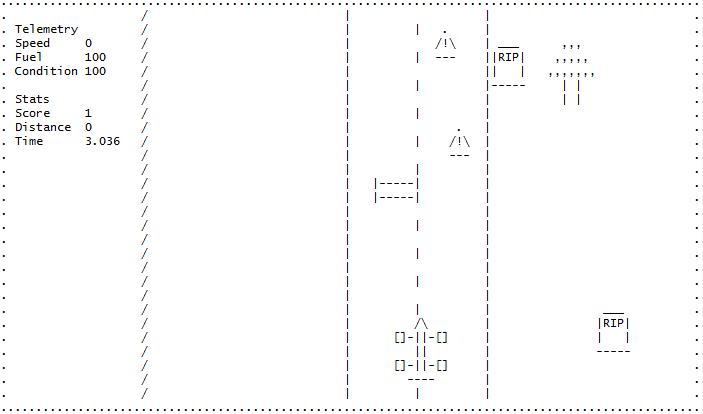
\includegraphics[width=0.667\paperwidth]{images/speed_testdecel0}
	\caption{Decelerating when speed is already zero}
	\label{fig:speed_testdecel0} 
	\end{center}
\end{figure}
\newline
This also shows that the fuel and distance are not modified while the car is stationary but the time keeps increasing. This means the function \emph{update\_game\_screen()} is doing it's job of choosing which parts of the game logic to update.
\newpage

\subsubsection*{Distance covered with different speeds}
Figure \ref{fig:speed_midspeed} shows the car travels 4 units in three seconds when speed is set to 5. Straight after, the speed was increased to 10 and Figure  \ref{fig:speed_maxspeed} shows the car travelled 10 units in three seconds.
\begin{figure}[!ht]
	\begin{center}
	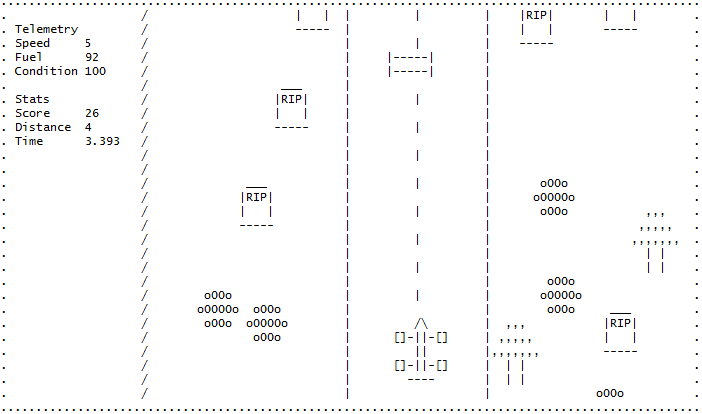
\includegraphics[width=0.667\paperwidth]{images/speed_midspeed}
	\caption{Distance covered at speed 5 after three seconds}
	\label{fig:speed_midspeed} 
	\end{center}
\end{figure}
\begin{figure}[!ht]
	\begin{center}
	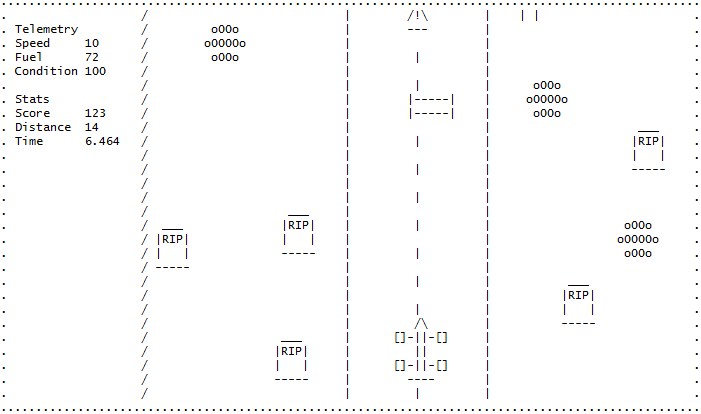
\includegraphics[width=0.667\paperwidth]{images/speed_maxspeed}
	\caption{Distance covered at speed 10 after three seconds}
	\label{fig:speed_maxspeed} 
	\end{center}
\end{figure}
\newpage

\subsubsection*{Speed does not go above 10}
This test was set up by having the car reach speed 10. Afterwards, the following keys were pressed "w,w,w,w" to verify that the speed wouldn't go above 10. 
\begin{figure}[!ht]
	\begin{center}
	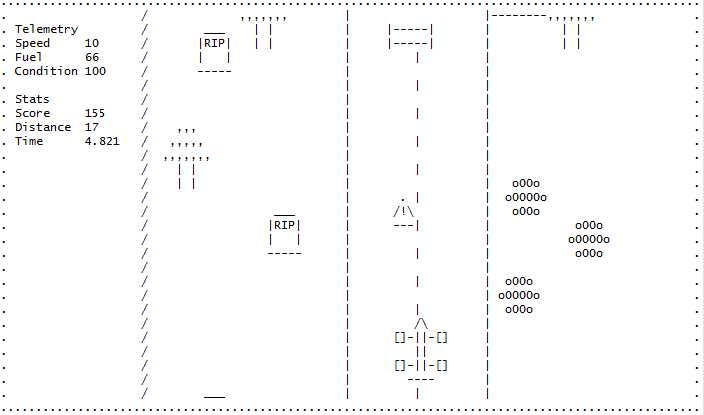
\includegraphics[width=0.667\paperwidth]{images/speed_test_maxacel10}
	\caption{Accelerating when speed is already 10}
	\label{fig:speed_test_acel10} 
	\end{center}
\end{figure}

\clearpage

%----------------------------------------------------------------------------------------
%	SCENERY AND OBSTACLES
%----------------------------------------------------------------------------------------
\section{Scenery and Obstacles}
In this game, obstacles can be separated into three categories.  Fuel depots have additional functionality and are covered in the section \emph{Fuel Depot}. 
\begin{itemize}
 	\item Terrain (spawns offroad)
 	\item Road Hazards (limited to the road)
	\item Fuel Depots
\end{itemize}

\subsection*{Globals}
\begin{lstlisting}[style=CStyle]
	// obstacles.h
	int max_terrain_obs;	
\end{lstlisting}
The maximum amount of terrain obstacles that can appear at one time. Dependant on the screen size.
\begin{lstlisting}[style=CStyle]
	// obstacles.h
	sprite_id *terrain;
\end{lstlisting}
An array that holds the ids of all sprites representing terrain.
\begin{lstlisting}[style=CStyle]
	// obstacles.h
	int max_hazards;
\end{lstlisting}
The maximum amount of road hazards that can appear at one time. 
\begin{lstlisting}[style=CStyle]
	// obstacles.h
	sprite_id *hazards;
\end{lstlisting}
An array that holds the ids of all sprites representing road hazards.
\begin{lstlisting}[style=CStyle]
	// imagemngr.h
	#define TERRAIN     0
	#define HAZARD      1
\end{lstlisting}
Used to define the different types of obstacles.
\begin{lstlisting}[style=CStyle]
	// imagemngr.h
	#define NUM_TERRAIN_TYPES	3
	#define TERRAIN_BOULDER		0
	#define TERRAIN_TREE 			1
	#define TERRAIN_GRAVE			2
\end{lstlisting}
Used to differentiate between the different types of terrain.
\begin{lstlisting}[style=CStyle]
	// imagemngr.h
	#define NUM_HAZARD_TYPES	2
	#define HAZARD_SPIKES			0
	#define HAZARD_TRIANGLE		1
\end{lstlisting}
Used to differentiate between the different types of road hazards.
\begin{lstlisting}[style=CStyle]
	// imagemngr.c
	char* terrain_image[NUM_TERRAIN_TYPES];
	int terrain_width[NUM_TERRAIN_TYPES];
	int terrain_height[NUM_TERRAIN_TYPES];
	char* hazards_image[NUM_HAZARD_TYPES];
	int hazards_width[NUM_HAZARD_TYPES];
	int hazards_height[NUM_HAZARD_TYPES];
\end{lstlisting}
Holds information about a sprite's bitmap for each different type of terrain and hazard.
\newpage

\subsection*{Functions}
\begin{lstlisting}[style=CStyle]
	// obstacles.c
	void init_obs();	
\end{lstlisting}
Allocate the required memory to the arrays which will hold all obstacles. Will also calculate the maximum number of obstacles that can appear in one go.
\begin{lstlisting}[style=CStyle]
	// obstacles.c
	void setup_obs();
\end{lstlisting}
Calls all of the required setup functions for obstacles, road, fuel station and the finish line.
\begin{lstlisting}[style=CStyle]
	// obstacles.c
	void setup_terrain();
\end{lstlisting}
Fills the terrain array with sprites and makes sure none are spawned on top of each other.
\begin{lstlisting}[style=CStyle]
	// obstacles.c
	void terrain_create(int index);
\end{lstlisting}
Called by \emph{setup\_terrain()}. Chooses a type of terrain and a random valid location for it. Then proceeds to add the sprite id of that terrain to the appropriate array.
\begin{lstlisting}[style=CStyle]
	// obstacles.c
	void terrain_reset(int index);
\end{lstlisting}
Moves the terrain corresponding to the index a randomised distance above the screen. The type of terrain and it's location will also be randomised. Nothing will happen if it collides with another obstacle so this function should be called again in the next game tick (done in \emph{update\_game\_screen()}.
\begin{lstlisting}[style=CStyle]
	// obstacles.c
	void update_terrain();
\end{lstlisting}
Steps all of the terrain sprites in the terrain array and then checks if any have gone out of bounds below the screen. Will then attempt to reset the terrain with \emph{terrain\_reset()}.
\begin{lstlisting}[style=CStyle]
	// obstacles.c
	void setup_hazards() 
\end{lstlisting}
Fills the hazards array with sprites and makes sure none are spawned on top of each other.
\begin{lstlisting}[style=CStyle]
	// obstacles.c
	void hazard_create(int index)
\end{lstlisting}
Called by \emph{setup\_hazards()}. Chooses a type of hazard and a random valid location for it. Then proceeds to add the sprite id of that hazard to the appropriate array.
\begin{lstlisting}[style=CStyle]
	// obstacles.c
	void hazard_reset(int index)
\end{lstlisting}
Moves the hazard corresponding to the index given a randomised distance above the screen. The type of hazard and it's location will also be randomised. Nothing will happen if it collides with another obstacle so this function should be called again in the next game tick (done in \emph{update\_game\_screen()}. The hazard and terrain setup, update and reset functions are similar but need to be separated due to different arrays being used and both having different limitations on where they can be spawned.
\begin{lstlisting}[style=CStyle]
	// obstacles.c
	void update_hazards();
\end{lstlisting}
Steps all of the hazard sprites in the hazards array and then checks if any have gone out of bounds below the screen. Will then attempt to reset the hazard with \emph{hazard\_reset()}.
\newpage
\begin{lstlisting}[style=CStyle]
	// obstacles.c
	void update_obs();
\end{lstlisting}
Call all of the update functions for each different type of obstacles.
\begin{lstlisting}[style=CStyle]
	// obstacles.c
	void draw_obs();
\end{lstlisting}
Call all of the draw functions for each different type of obstacles.
\begin{lstlisting}[style=CStyle]
	// obstacles.c
	void draw_terrain();
\end{lstlisting}
Call \emph{sprite\_draw()} for each terrain in the terrain array.
\begin{lstlisting}[style=CStyle]
	// obstacles.c
	void draw_hazards();
\end{lstlisting}
Call \emph{sprite\_draw()} for each hazard in the hazards array.
\begin{lstlisting}[style=CStyle]
	// imagemngr.c
	void imagemngr_init();
\end{lstlisting}
Call the appropriate init function for each type of obstacle.
\begin{lstlisting}[style=CStyle]
	// imagemngr.c
	void hazards_init();
\end{lstlisting}
Add all of the hazard bitmap information to the appropriate arrays.
\begin{lstlisting}[style=CStyle]
	// imagemngr.c
	void terrain_init();
\end{lstlisting}
Add all of the terrain bitmap information to the appropriate arrays.
\begin{lstlisting}[style=CStyle]
	// imagemngr.c
	void add_image(int id, char* image, int width, int height, int type);
\end{lstlisting}
Add the bitmap information of a specific sprite to the appropriate array (defined by the \emph{type} variable).
\begin{lstlisting}[style=CStyle]
	// imagemngr.c
	char* get_image(int id, int type, int* width, int* height);
\end{lstlisting}
Get the bitmap and its properties from the appropriate array defined by the \emph{type} variable.

\newpage

\subsection*{Testing}
\subsubsection*{Obstacles scroll at intermediate speed}
After the game is started, the gravestone in the top-right in Figure \ref{fig:obs_test_midspeedscroll} is taken as a reference point. The car is then accelerated to a speed of 5 the time it takes for the reference to reach the bottom of the screen shown in Figure \ref{fig:obs_test_midspeedscroll2} is found to be about 4 seconds.
\begin{figure}[!ht]
	\begin{center}
	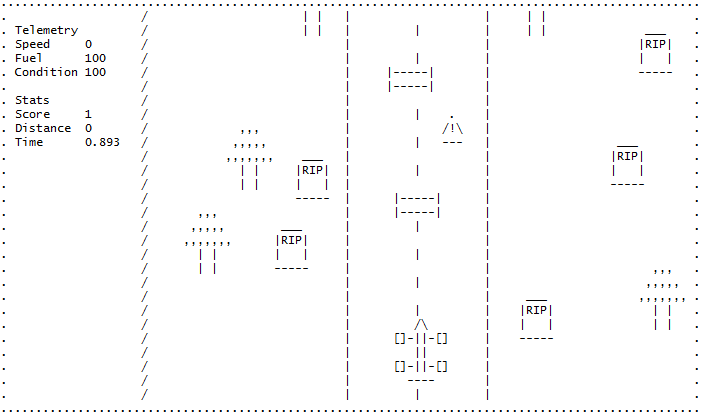
\includegraphics[width=0.63\paperwidth]{images/obs_test_midspeedscroll}
	\caption{Calculating time for scenery to scroll past (top-right gravestone is reference point)}
	\label{fig:obs_test_midspeedscroll} 
	\end{center}
\end{figure}
\begin{figure}[!ht]
	\begin{center}
	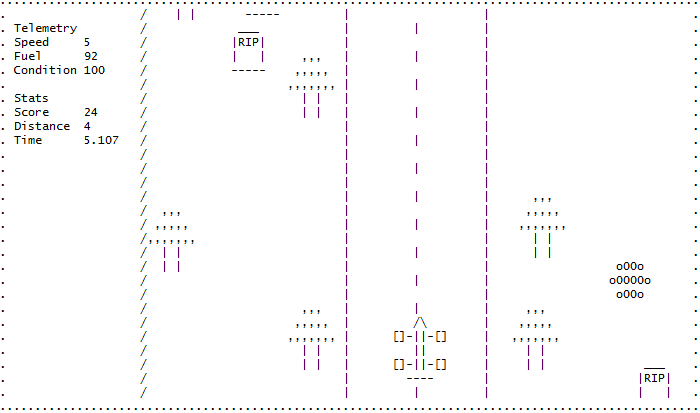
\includegraphics[width=0.63\paperwidth]{images/obs_test_midspeedscroll2}
	\caption{Calculating time for scenery to scroll past (reference gravestone scrolling out of view)}
	\label{fig:obs_test_midspeedscroll2} 
	\end{center}
\end{figure}
\newpage
\subsubsection*{Obstacles scroll at max speed}
The acceleration input is pressed until the car reaches max speed. The boulder at the top right of the screen is taken as a reference point. Figure \ref{fig:obs_test_maxspeedscroll2} shows that it took 1 second for the boulder to reach the bottom of the screen. Both tests also show scenery scrolling in, middle and scrolling out in the screen.
\begin{figure}[!ht]
	\begin{center}
	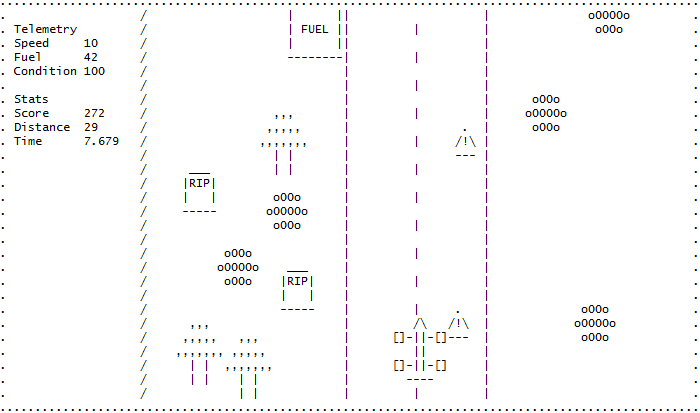
\includegraphics[width=0.63\paperwidth]{images/obs_test_maxspeedscroll}
	\caption{Calculating time for scenery to scroll past (top-right boulder is reference point)}
	\label{fig:obs_test_maxspeedscroll} 
	\end{center}
\end{figure}
\begin{figure}[!ht]
	\begin{center}
	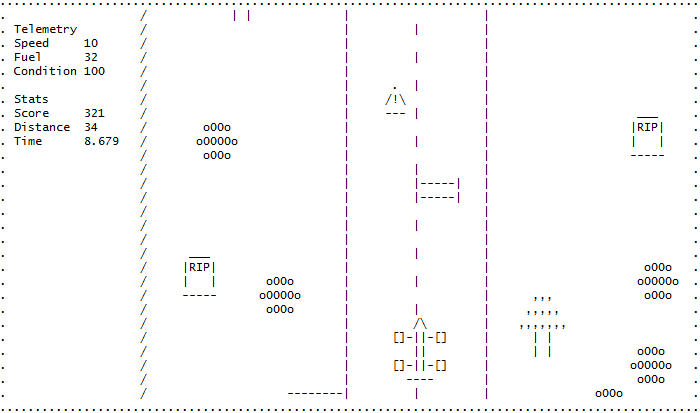
\includegraphics[width=0.63\paperwidth]{images/obs_test_maxspeedscroll2}
	\caption{Calculating time for scenery to scroll past (only top can reference boulder can be seen)}
	\label{fig:obs_test_maxspeedscroll2} 
	\end{center}
\end{figure}
\clearpage

%----------------------------------------------------------------------------------------
%	FUEL DEPOT
%----------------------------------------------------------------------------------------
\section{Fuel Depot}
The Fuel Depot is a type of obstacle that refuels the player's car if it is parked for 3 seconds directly next to it. To smooth out the gameplay, the player will automatically park the car if they're travelling at a speed of 2 or less. A collision with the fuel depot will immediately end the game for the player, regardless of the car's condition.

\subsection*{Globals}
\begin{lstlisting}[style=CStyle]
	// obstacles.h
	#define FUEL_STATION_DELAY_DIST	30
\end{lstlisting}
The minimum distance which the next fuel depot can appear after the old one leaves the playing area. 
\begin{lstlisting}[style=CStyle]
	// obstacles.h
	#define FUEL_STATION_VARIANCE	15
\end{lstlisting}
The variance in distance that the next fuel depot will spawn at. When we combine with \emph{FUEL\_STATION\_DELAY\_DIST}, we know that a fuel depot will spawn between 30 and 45 units of distance above the screen after the old depot leaves the playing area. 
\begin{lstlisting}[style=CStyle]
	// obstacles.h
	sprite_id fuel_station;
\end{lstlisting}
The sprite which represents the fuel depot.
\newline

\subsection*{Functions}
\begin{lstlisting}[style=CStyle]
	// obstacles.c
	void setup_fuel_station();
\end{lstlisting}
Creates the fuel depot sprite and places it in its initial position. Will also randomly choose a random side of the road to place it in. 
\begin{lstlisting}[style=CStyle]
	// obstacles.c
	void update_fuel_station();
\end{lstlisting}
Will step the sprite for the fuel depot and then check if it went out of bounds. If it has, it will reset the fuel station to a random location (limted by the globals) above the playing area and a random side of the road. Will then reset any terrain that was in the way to avoid overlap. 
\newline

\newpage
\subsection*{Testing}
\subsubsection*{Fuel Depot scrolls at intermediate speed}
The game is played with the car kept at a constant speed of 5. Figures \ref{fig:fueldepot_test_midspeed} and \ref{fig:fueldepot_test_midspeed2} show that it took the fuel depot about three seconds to scroll past the playing area.
\begin{figure}[!ht]
	\begin{center}
	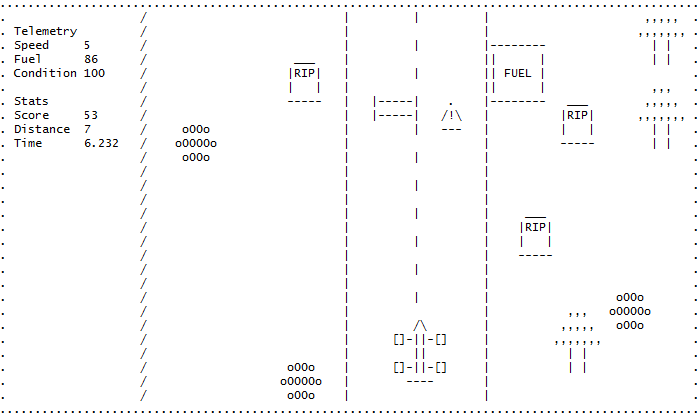
\includegraphics[width=0.63\paperwidth]{images/fueldepot_test_midspeed}
	\caption{Calculating time for fuel depot to scroll past at speed of 5}
	\label{fig:fueldepot_test_midspeed} 
	\end{center}
\end{figure}
\begin{figure}[!ht]
	\begin{center}
	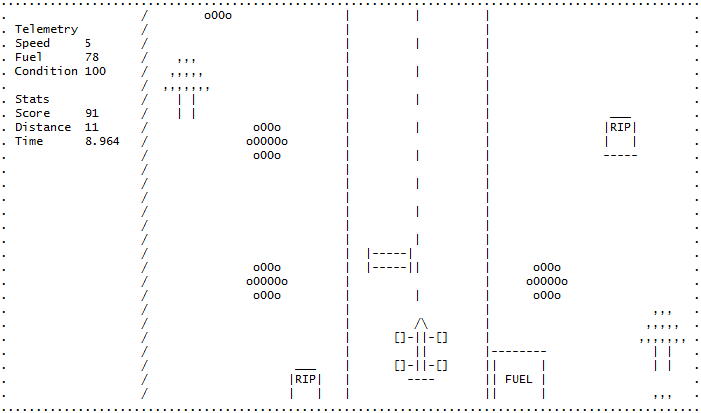
\includegraphics[width=0.63\paperwidth]{images/fueldepot_test_midspeed2}
	\caption{Calculating time for fuel depot to scroll past at speed of 5}
	\label{fig:fueldepot_test_midspeed2} 
	\end{center}
\end{figure}
\newpage
\subsubsection*{Fuel Depot scrolls at maximum speed}
The game is played with the car kept at a constant speed of 10. Figures \ref{fig:fueldepot_test_maxspeed} and \ref{fig:fueldepot_test_maxspeed2} show that it took the fuel depot about one second to scroll past the playing area. Both of these tests show that the fuel depot is scrolling at the same rate as the rest of the scenery and obstacles.  As seen in Figures \ref{fig:car_test_rightborder} and \ref{fig:car_test_leftborder}, the fuel depot can also spawn on any side of the road.
\begin{figure}[!ht]
	\begin{center}
	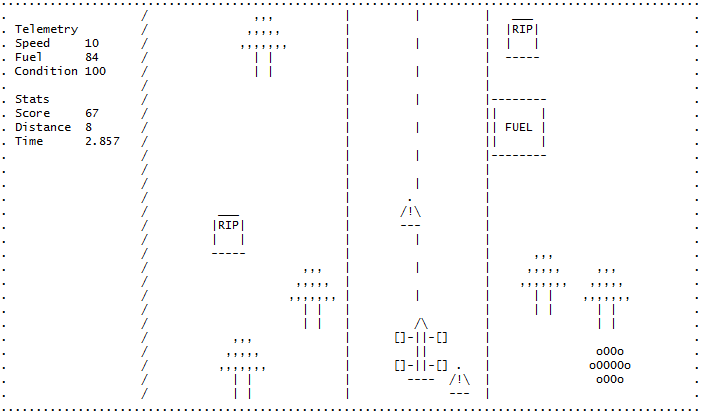
\includegraphics[width=0.63\paperwidth]{images/fueldepot_test_maxspeed}
	\caption{Calculating time for fuel depot to scroll past at speed of 5}
	\label{fig:fueldepot_test_maxspeed} 
	\end{center}
\end{figure}
\begin{figure}[!ht]
	\begin{center}
	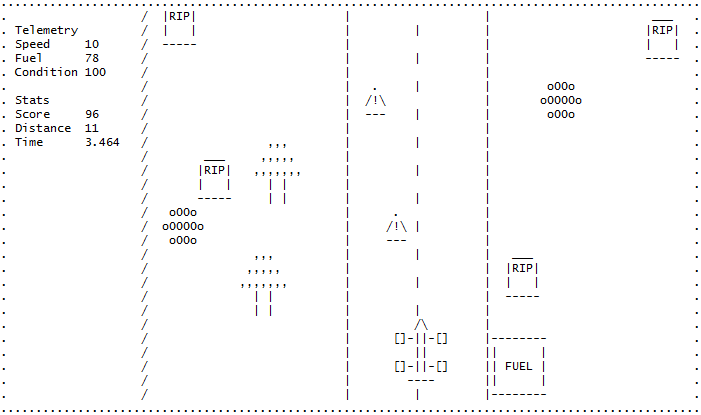
\includegraphics[width=0.63\paperwidth]{images/fueldepot_test_maxspeed2}
	\caption{Calculating time for fuel depot to scroll past at speed of 10}
	\label{fig:fueldepot_test_maxspeed2} 
	\end{center}
\end{figure}
\clearpage

%----------------------------------------------------------------------------------------
%	FUEL
%----------------------------------------------------------------------------------------
\section{Fuel}
The car start with a fuel tank which decreases as it moves. The faster it moves, the faster the fuel is depleted. After parking next to a fuel depot for 3 seconds, the fuel tank is refilled to max. The fuel tank can also be refilled to max after a collision with an obstacle. 

\subsection*{Globals}
\begin{lstlisting}[style=CStyle]
	// zombiemountain.h
	int fuel;
\end{lstlisting}
The current amount of fuel available to the player.
\begin{lstlisting}[style=CStyle]
	// zombiemountain.h
	bool refuelling;
\end{lstlisting}
Represents whether the car is currently refuelling.
\begin{lstlisting}[style=CStyle]
	// zombiemountain.h
	timer_id refuel_timer;
\end{lstlisting}
A timer that is used to verify that the car has remained next to the fuel depot for 3 seconds.
\newline

\subsection*{Functions}
\begin{lstlisting}[style=CStyle]
	// main.c
	void check_refuel();
\end{lstlisting}
Checks if the car meets all of the criteria to begin refuelling (next to a fuel station and travelling at a speed of 2 or less). Then switches the \emph{refuelling} variable to true, sets speed to 0 and starts \emph{refuel\_timer}.
\begin{lstlisting}[style=CStyle]
	// main.c
	void refuel();
\end{lstlisting}
Called every tick of the game loop. If the car isn't already refuelling, call the \emph{check\_refuel()}. Otherwise it will make sure the car's speed has remained at 0. If the \emph{refuel\_timer} has expirer, it'll refill the fuel tank and release the car at a speed of 1.
\begin{lstlisting}[style=CStyle]
	// main.c
	void update_game_screen();
\end{lstlisting}
Will check if the fuel is above 0 and will give the game over message when the fuel tank is empty.

\newpage
\subsection*{Testing}
\subsubsection*{Fuel loss moving at intermediate speed}
The car is kept at a constant speed of 5 for three seconds. Figures \ref{fig:fuel_test_lossmidspeed} and \ref{fig:fuel_test_lossmidspeed2} show that the car loses 8 fuel units after 3 seconds at intermediate speed. Figure \ref{fig:speed_testdecel0} also shows that the car doesn't lose fuel while remaining stationary.
\begin{figure}[!ht]
	\begin{center}
	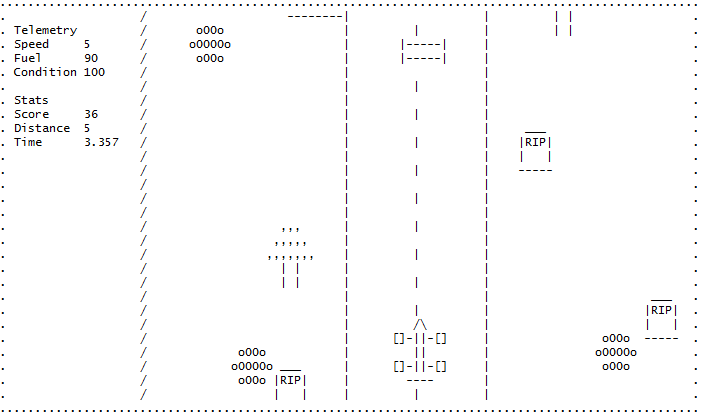
\includegraphics[width=0.63\paperwidth]{images/fuel_test_lossmidspeed}
	\caption{Calculating fuel loss at intermediate speed}
	\label{fig:fuel_test_lossmidspeed} 
	\end{center}
\end{figure}
\begin{figure}[!ht]
	\begin{center}
	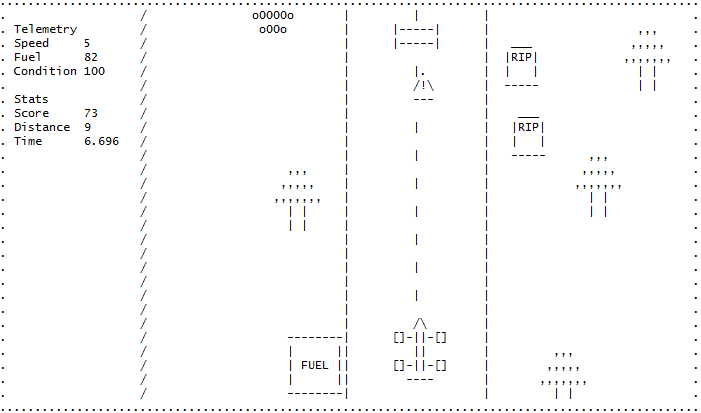
\includegraphics[width=0.63\paperwidth]{images/fuel_test_lossmidspeed2}
	\caption{Calculating fuel loss at intermediate speed}
	\label{fig:fuel_test_lossmidspeed2} 
	\end{center}
\end{figure}
\newpage
\subsubsection*{Fuel loss moving at max speed}
The car is kept at a constant speed of 10 for three seconds. Figures \ref{fig:fuel_test_lossmaxspeed} and \ref{fig:fuel_test_lossmaxspeed2} show that the car loses 30 fuel units after 3 seconds at maximum speed. 
\begin{figure}[!ht]
	\begin{center}
	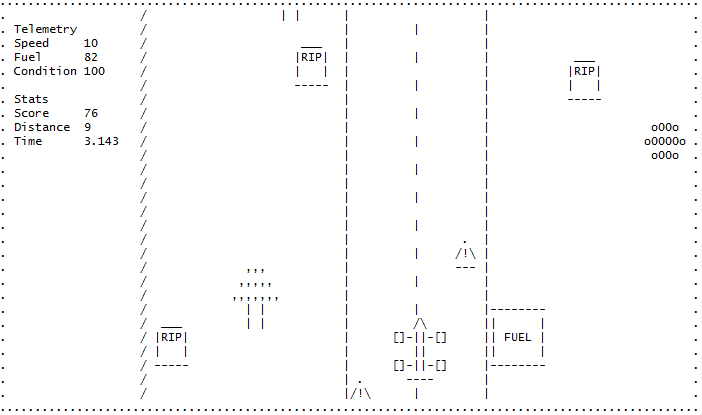
\includegraphics[width=0.63\paperwidth]{images/fuel_test_lossmaxspeed}
	\caption{Calculating fuel loss at max speed}
	\label{fig:fuel_test_lossmaxspeed} 
	\end{center}
\end{figure}
\begin{figure}[!ht]
	\begin{center}
	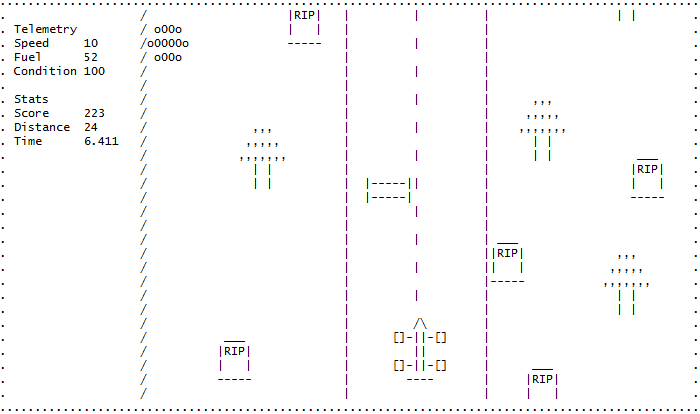
\includegraphics[width=0.63\paperwidth]{images/fuel_test_lossmaxspeed2}
	\caption{Calculating fuel loss at max speed}
	\label{fig:fuel_test_lossmaxspeed2} 
	\end{center}
\end{figure}
\newpage
\subsubsection*{Refuelling}
\begin{figure}[!ht]
	\begin{center}
	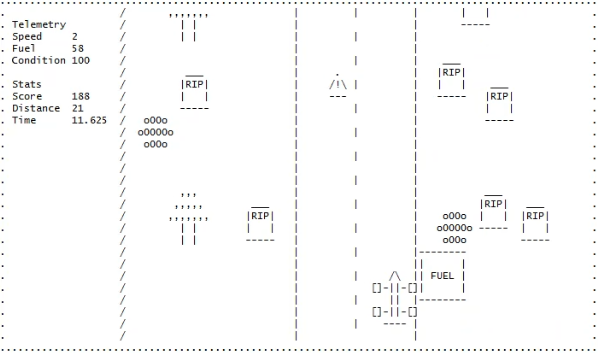
\includegraphics[width=0.63\paperwidth]{images/fuel_test_refuelapproach}
	\caption{Car approaching the fuel station}
	\label{fig:fuel_test_refuelapproach} 
	\end{center}
\end{figure}
\begin{figure}[!ht]
	\begin{center}
	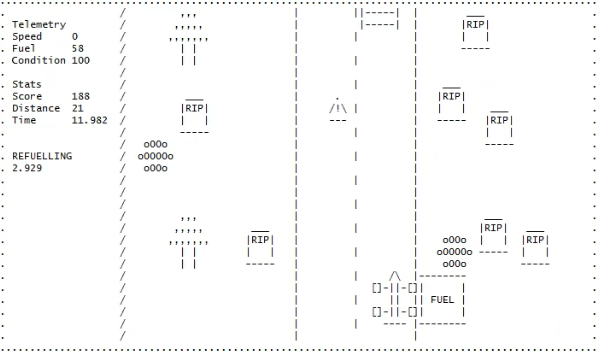
\includegraphics[width=0.63\paperwidth]{images/fuel_test_refuelbegin}
	\caption{Car is stopped automatically and refuelling begins}
	\label{fig:fuel_test_refuelbegin} 
	\end{center}
\end{figure}
\newpage
\begin{figure}[!ht]
	\begin{center}
	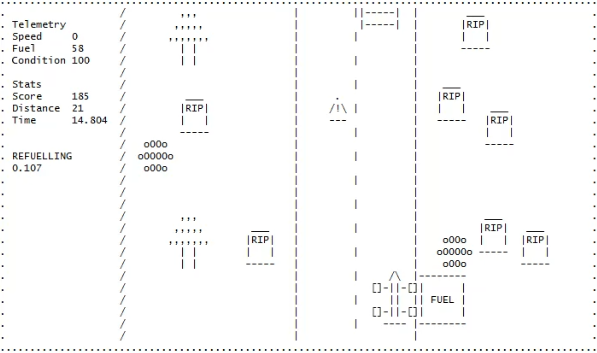
\includegraphics[width=0.63\paperwidth]{images/fuel_test_refuelend}
	\caption{Time has passed and the player is waiting for refuel to finish}
	\label{fig:fuel_test_refuelend} 
	\end{center}
\end{figure}
\begin{figure}[!ht]
	\begin{center}
	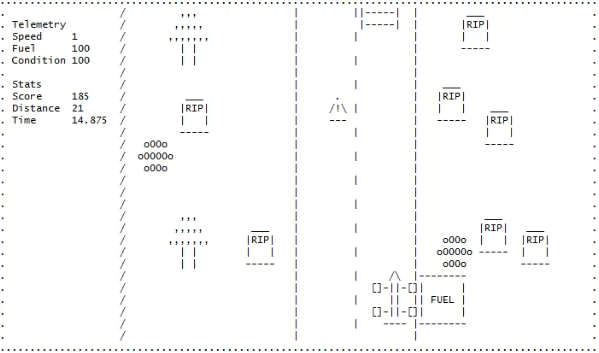
\includegraphics[width=0.63\paperwidth]{images/fuel_test_refuelrelease}
	\caption{Refuelling ended, fuel tank is topped up and the car is released at a speed of 1}
	\label{fig:fuel_test_refuelrelease} 
	\end{center}
\end{figure}

\clearpage

%----------------------------------------------------------------------------------------
%	DISTANCE TRAVELLED
%----------------------------------------------------------------------------------------
\section{Distance Travelled}
\subsection*{Globals}
\begin{lstlisting}[style=CStyle]
	// zombiemountain.h
	int distance_counter;
\end{lstlisting}
A counter that decides when to increment the distance travelled by the car. Currently, the distance is incremented after the scenery scrolls for 5 ticks.
\begin{lstlisting}[style=CStyle]
	// zombiemountain.h
	int distance_travelled;
\end{lstlisting}
Represents the units of distance travelled by the car since the game started. 
\begin{lstlisting}[style=CStyle]
	// obstacles.h
	sprite_id finish_line;
\end{lstlisting}
The sprite that represents the finish line.
\begin{lstlisting}[style=CStyle]
	// obstacles.h
	#define FINISH_LINE_DIST	500
\end{lstlisting}
How many units above the screen the finish line will be spawned (not to be confused with the distance it'll be spawned at). 
\newline

\subsection*{Functions}
\begin{lstlisting}[style=CStyle]
	// main.c
	void update_distance();
\end{lstlisting}
Called everytime the car moves. It'll increment the \emph{distance\_counter} and increment the distance travelled when the counter passes a threshold.
\begin{lstlisting}[style=CStyle]
	// imagemngr.c
	char* get_finish_line_image();
\end{lstlisting}
Returns the bitmap which represens the finish line.
\begin{lstlisting}[style=CStyle]
	// obstacles.c
	void setup_finish_line();
\end{lstlisting}
Creates the finish line sprite and spawns it above the screen.
\begin{lstlisting}[style=CStyle]
	// main.c
	void update_game_screen();
\end{lstlisting}
Will check if the player has crossed the finish line sprite and if so, change to the game over screen. 
\newline

\subsection*{Testing}
\subsubsection*{Distance covered proportional to speed}
Figure \ref{fig:speed_testdecel0} shows that the distance counter is not incremented when the car is at a speed of 0.
\newline
Figure \ref{fig:speed_midspeed} shows the car travels 4 units in three seconds when the speed is 5.
\newline
Figure \ref{fig:speed_maxspeed} shows that the car travels 10 units in three seconds when the speed is 10. 
\newpage
\subsubsection*{Game finishes when car crosses the finish line}
The game was played normally and a screenshot was taken just as the player crossed the finish line. Figure \ref{fig:finishline_test_win2} shows what the screen looks like the next frame.
\begin{figure}[!ht]
	\begin{center}
	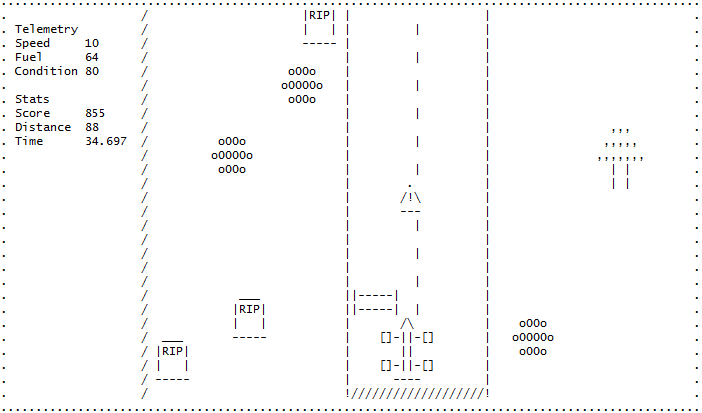
\includegraphics[width=0.63\paperwidth]{images/finishline_test_win}
	\caption{Crossing the finish line during normal gameplay}
	\label{fig:finishline_test_win} 
	\end{center}
\end{figure}
\begin{figure}[!ht]
	\begin{center}
	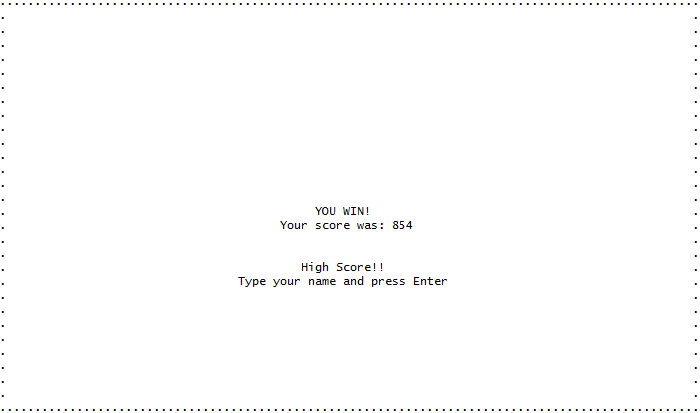
\includegraphics[width=0.63\paperwidth]{images/finishline_test_win2}
	\caption{The next frame after crossing the finish line}
	\label{fig:finishline_test_win2} 
	\end{center}
\end{figure}
\clearpage


%----------------------------------------------------------------------------------------
%	COLLISION
%----------------------------------------------------------------------------------------
\section{Collision}
Collision uses simple bounding box detection. The car is reset and the condition reduced if the car hits an obstacle head on. The car's horizontal movement is stopped if it tries to move into an obstacle. 

\subsection*{Globals}
\begin{lstlisting}[style=CStyle]
	// obstacles.h
	int car_condition;
\end{lstlisting}
The only global added by this section. Collision detection makes use mostly of globals already implemented when the scenery is created. 
\newline

\subsection*{Functions}
\begin{lstlisting}[style=CStyle]
	// obstacles.c
	bool check_collision(sprite_id sprite);
\end{lstlisting}
Iterates through every obstacle in the game and checks if the sprite passed to this function collides with any of therm.
\begin{lstlisting}[style=CStyle]
	// obstacles.c
	bool check_sprite_collided(sprite_id sprite1, sprite_id sprite2);
\end{lstlisting}
Checks if the two sprites passed to this function collide with each other.
\begin{lstlisting}[style=CStyle]
	// main.c
	void update_game_screen();
\end{lstlisting}
Will check if the player has collided with any object every time the car moves. Will also check if the car has collided with a fuel depot and throw the game over dialogue if it has.
\begin{lstlisting}[style=CStyle]
	// main.c
	void handle_collision();
\end{lstlisting}
When it's found that the player has collided with an object that is not the fuel depot, this function will reset the location of the player and clear any hazards on the way while also reducing the car's condition nad changing to the game over screen if it reaches 0.
\newpage

\subsection*{Testing}
\subsubsection*{Head on collision with road hazards}
The car is moved head on into a collision with a road hazard and the result screenshotted. As there were no hazards blocking the path of the car when it reset, no obstacles were required to be reset.
\begin{figure}[!ht]
	\begin{center}
	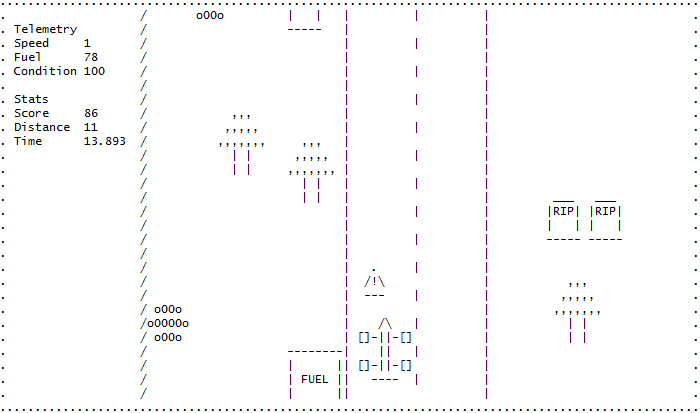
\includegraphics[width=0.63\paperwidth]{images/collision_test_headon}
	\caption{The player a few frames before crashing into a road hazard}
	\label{fig:collision_test_headon} 
	\end{center}
\end{figure}
\begin{figure}[!ht]
	\begin{center}
	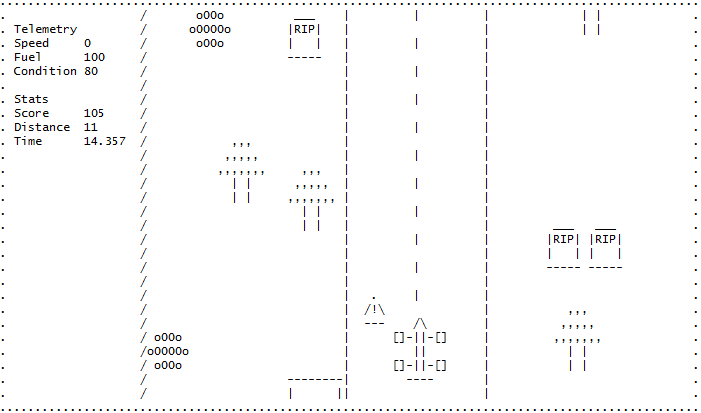
\includegraphics[width=0.63\paperwidth]{images/collision_test_headon2}
	\caption{The player immediately after crashing into a road hazard}
	\label{fig:collision_test_headon2} 
	\end{center}
\end{figure}
\newpage
\subsubsection*{Head on collision with terrain}
The car is moved into a collision course with a piece of terrain. The resulting screen in Figure \ref{fig:collision_test_headon_terrain2} shows that the triangle hazard had to be reset in order for the car to be placed in its starting location.
\begin{figure}[!ht]
	\begin{center}
	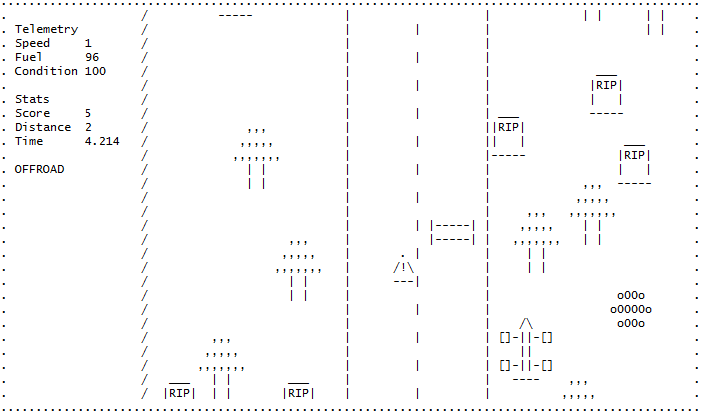
\includegraphics[width=0.63\paperwidth]{images/collision_test_headon_terrain}
	\caption{The player a few frames before crashing into terrain}
	\label{fig:collision_test_headon_terrain} 
	\end{center}
\end{figure}
\begin{figure}[!ht]
	\begin{center}
	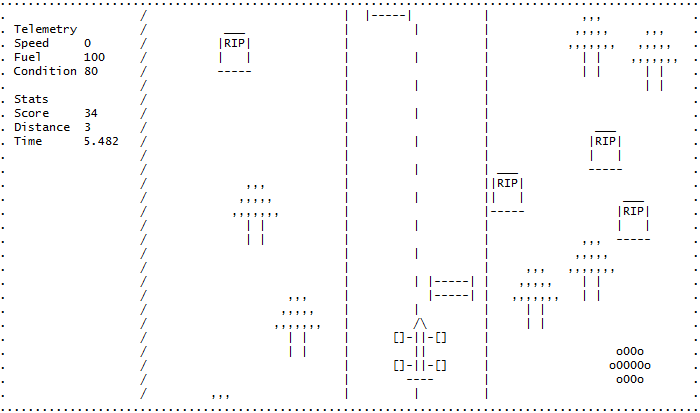
\includegraphics[width=0.63\paperwidth]{images/collision_test_headon_terrain2}
	\caption{The player immediately after crashing into terrain}
	\label{fig:collision_test_headon_terrain2} 
	\end{center}
\end{figure}
\newpage
\subsubsection*{Head on collision with fuel depot}
The car is moved into a collision course with a piece of terrain. The resulting screen in Figure \ref{fig:collision_test_headon_terrain2} shows that the triangle hazard had to be reset in order for the car to be placed in its starting location.
\begin{figure}[!ht]
	\begin{center}
	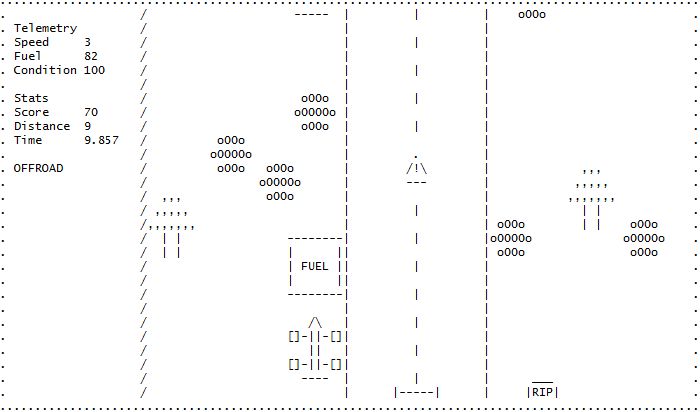
\includegraphics[width=0.63\paperwidth]{images/collision_test_headon_depot}
	\caption{The player a few frames before crashing into a fuel depot}
	\label{fig:collision_test_headon_depot} 
	\end{center}
\end{figure}
\begin{figure}[!ht]
	\begin{center}
	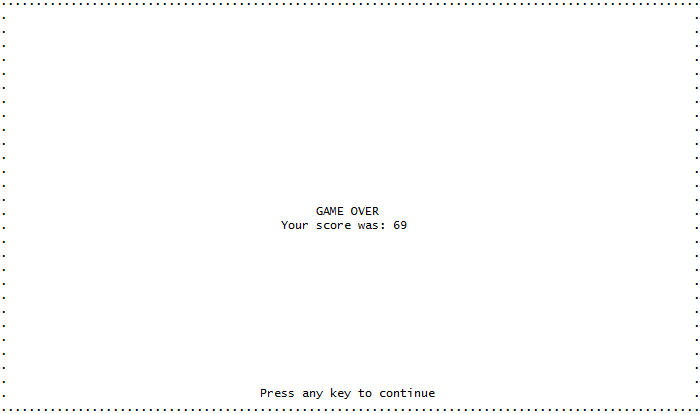
\includegraphics[width=0.63\paperwidth]{images/collision_test_headon_depot2}
	\caption{The screen that shows straight after the player crashes into a fuel depot}
	\label{fig:collision_test_headon_depot2} 
	\end{center}
\end{figure}
\newpage
\subsubsection*{Side collision}
This test involved attempting to crash into an obstacle sideways. In Figure \ref{fig:collision_test_side} the car was moved next to the tree and the following input commands were given - "a,a,a". For Figure \ref{collision_test_side2}, the car was moved next to the fence hazard and the following input commands were given - "d,d,d". This shows how the car's movement is restricted if it would collide sideways with an obstacle.
\begin{figure}[!ht]
	\begin{center}
	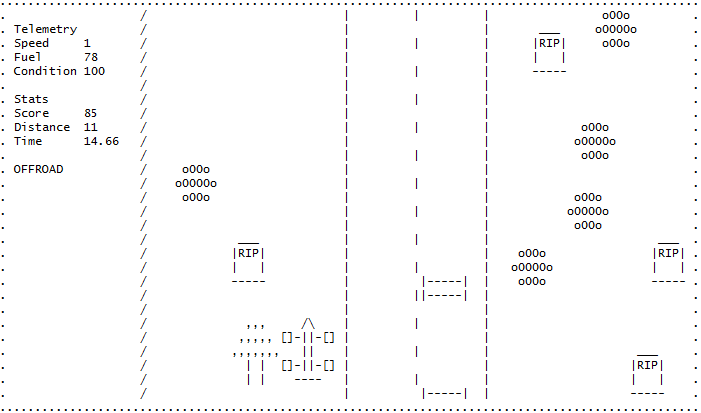
\includegraphics[width=0.63\paperwidth]{images/collision_test_side}
	\caption{Attempting to move to the left next to an obstacle}
	\label{fig:collision_test_side} 
	\end{center}
\end{figure}
\begin{figure}[!ht]
	\begin{center}
	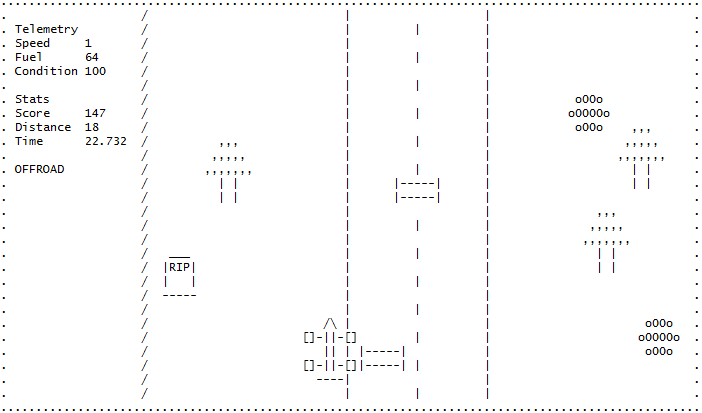
\includegraphics[width=0.63\paperwidth]{images/collision_test_side2}
	\caption{Attempting to move to the right next to an obstacle}
	\label{fig:collision_test_side2} 
	\end{center}
\end{figure}

\clearpage


%----------------------------------------------------------------------------------------
%	GAME OVER DIALOGUE
%----------------------------------------------------------------------------------------
\section{Game Over Dialogue}
The game over dialogue is given when the player has either won the game by crossing the finish line or lost by crashing into an obstacle or running out of fuel. 

\subsection*{Globals}
\begin{lstlisting}[style=CStyle]
	// zombiemountain.h
	bool game_over_loss;
\end{lstlisting}
Represents if the game was over either through a loss (true) or win (false).
\newline

\subsection*{Functions}
\begin{lstlisting}[style=CStyle]
	// main.c
	void update_game_over_screen();
\end{lstlisting}
Will change to the highscore screen if the user presses any key. Will also do some work if the user has a new highscore (explained in the section \emph{Part B - Highscore Screen}).
\begin{lstlisting}[style=CStyle]
	// main.c
	void draw_game_over_screen();
\end{lstlisting}
Will draw the to the screen a prompt saying if the player won or los as well as the score achieved. 
\newline

\subsection*{Testing}
\subsubsection*{Game over screens for win and loss}
Figures \ref{fig:finishline_test_win} and \ref{fig:finishline_test_win2} show the appearance of the game over screen when a player wins the game.
\newline
Figures \ref{fig:collision_test_headon_depot} and \ref{fig:collision_test_headon_depot2} show the resulting game over screen for when the player loses the game through any of the methods specified in the introduction of this section.
\newline
Figure \ref{fig:gameover_test_playagain} shows that the player can restart the game by pressing "p" or "s".
\begin{figure}[!ht]
	\begin{center}
	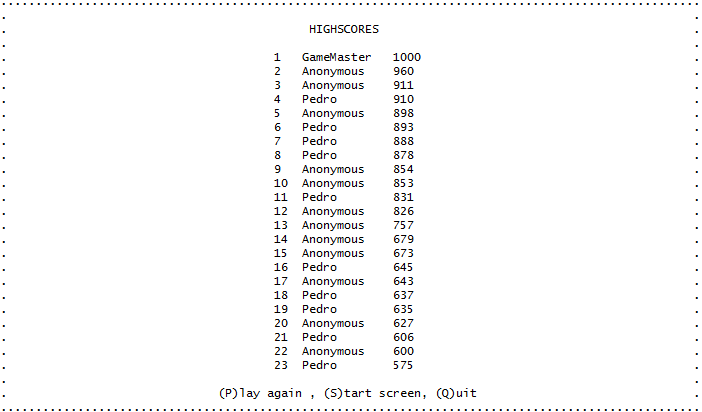
\includegraphics[width=0.6\paperwidth]{images/gameover_test_playagain}
	\caption{The highscore screen which shows how the player can restart the game}
	\label{fig:gameover_test_playagain} 
	\end{center}
\end{figure}

\clearpage

%----------------------------------------------------------------------------------------
%	PARTB
%----------------------------------------------------------------------------------------
\section{Part B - Highscore Screen}
The extension to my game is a highscore table. The top 100 highscores will be stored in a file called \emph{highscores} located in the game's directory. Whenever the player finished the game (by win or loss), if their score is high enough to be in the top 100, they will be prompted to type their name and their score will be added to the table.
\newline
The number of scores that can be show is dependant on the size of the screen. Up to 100 scores can be shown in the highscore screen. 
\newline
If the players chooses to not type anything when prompted for their name, \emph{Anonymous} will be written as the holder of that score. The player \emph{GameMaster} will always be shown to have 1000 points and provides the incentive for the player to take the number 1 spot.

\subsection*{Globals}
\begin{lstlisting}[style=CStyle]
	// hscore.h
	#define MAX_SCORES      100
\end{lstlisting}
The maximum number of scores we can display.
\begin{lstlisting}[style=CStyle]
	// hscore.h
	#define MAX_NAME_SIZE   12
\end{lstlisting}
The maximum number of characters a name can have.
\begin{lstlisting}[style=CStyle]
	// hscore.h
	int score;
\end{lstlisting}
The score the player has achieved.
\begin{lstlisting}[style=CStyle]
	// hscore.h
	char hscore_names[MAX_SCORES][MAX_NAME_SIZE+1];
\end{lstlisting}
The names of the top 100 playes are parsed from the \emph{highscores} file to this array
\begin{lstlisting}[style=CStyle]
	// hscore.h
	int hscore_scores[MAX_SCORES];
\end{lstlisting}
The scores of the top 100 playes are parsed from the \emph{highscores} file to this array
\newpage

\subsection*{Functions}
\begin{lstlisting}[style=CStyle]
	// main.c
	void draw_highscore_screen();
\end{lstlisting}
Draws the title of the screen and the prompts which ask the play what to do next. Will call \emph{draw\_hscores} to draw the highscore table.
\begin{lstlisting}[style=CStyle]
	// hscore.c
	void draw_hscores();
\end{lstlisting}
Draw the highscore table by deciding how many entries can be displayed on the screen. 
\begin{lstlisting}[style=CStyle]
	// main.c
	void update_highscore_screen();
\end{lstlisting}
Will change the game state to either the game, start or exit screen depending on the key pressed by the user.
\begin{lstlisting}[style=CStyle]
	// hscore.c
	void get_hscores();
\end{lstlisting}
Parses all of the data in the \emph{highscores} file and adds them to the appropriate arrays. Closes the connection to the file after.
\begin{lstlisting}[style=CStyle]
	// hscore.c
	void sort_scores();
\end{lstlisting}
Sorts the highscore table in descending order. Needed as \emph{process\_hscore()} add the new entry to the bottom of the table.
\begin{lstlisting}[style=CStyle]
	// hscore.c
	void process_hscore(char *name);
\end{lstlisting}
Add the current value of the \emph{score} variable to the highscore table under the name passed to the function. Also removes the lowest score if the table is already full with 100 highscores.
\begin{lstlisting}[style=CStyle]
	// hscore.c
	bool check_new_hscore();
\end{lstlisting}
Checks if there is a free spot on the highscore table or if the current score is higher than the lowest score in the table.
\begin{lstlisting}[style=CStyle]
	// hscore.c
	void save_scores();
\end{lstlisting}
Saves the highscore data from the arrays to the \emph{highscores} file in the format \emph{NAME SCORE newline}
\begin{lstlisting}[style=CStyle]
	// main.c
	void update_game_over_screen();
\end{lstlisting}
If there is a new highscore, it'll get the characters the user presses and add that to the name to be passed to the \emph{process\_hscore(name)} function. After the user presses \emph{ENTER}, the screen is changed to the highscore screen and the score is sent to be processed. 

\newpage
\subsection*{Testing}
\subsubsection*{Score is added with the right name}
The key "p" is pressed straight after the screen in \ref{fig:gameover_test_playagain} is displayed. After a full winning run of the game, the score earned is displayed in Figure \ref{fig:hscore_test_name}. The characters typed straight after this screen is shown is "NameTestENTER". Figure \ref{fig:hscore_test_name2} shows that the score and name were entered correctly and in the right location.
\begin{figure}[!ht]
	\begin{center}
	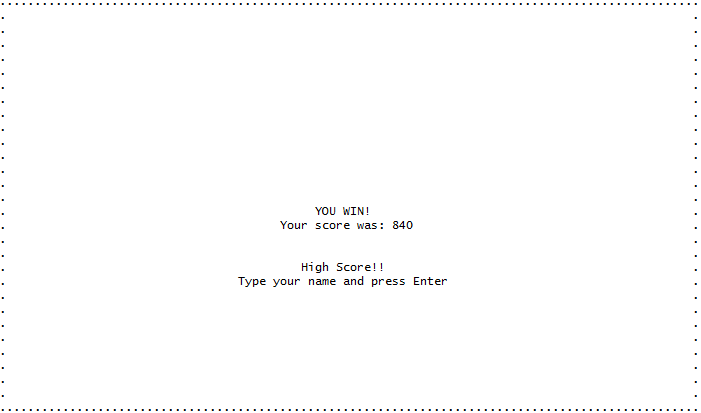
\includegraphics[width=0.6\paperwidth]{images/hscore_test_name}
	\caption{The score after winning the game}
	\label{fig:hscore_test_name} 
	\end{center}
\end{figure}
\begin{figure}[!ht]
	\begin{center}
	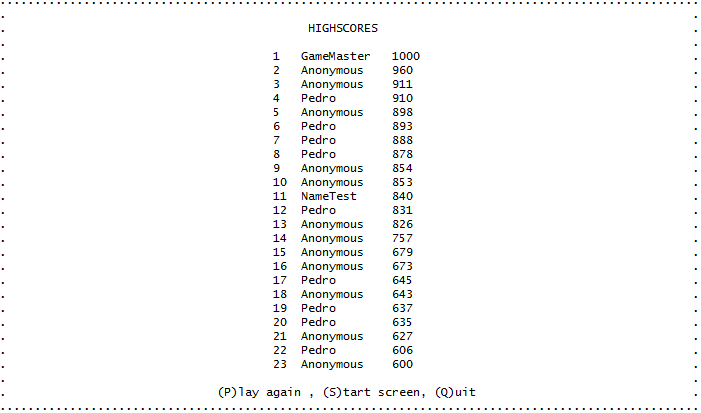
\includegraphics[width=0.6\paperwidth]{images/hscore_test_name2}
	\caption{The score and name are displayed correctly and in the right order}
	\label{fig:hscore_test_name2} 
	\end{center}
\end{figure}
\newpage
\subsubsection*{Score is added with no name typed}
The same setup was done as the previous test. However in the screen show in Figure \ref{fig:hscore_test_noname}, only ENTER was pressed. Figure \ref{fig:hscore_test_noname2} shows that the score earned beforehand of 873 is now in the table under the name "Anonymous".
\begin{figure}[!ht]
	\begin{center}
	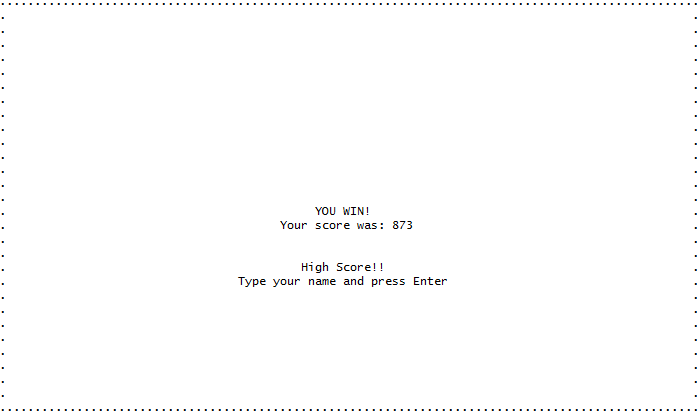
\includegraphics[width=0.6\paperwidth]{images/hscore_test_noname}
	\caption{The score after winning the game}
	\label{fig:hscore_test_noname} 
	\end{center}
\end{figure}
\begin{figure}[!ht]
	\begin{center}
	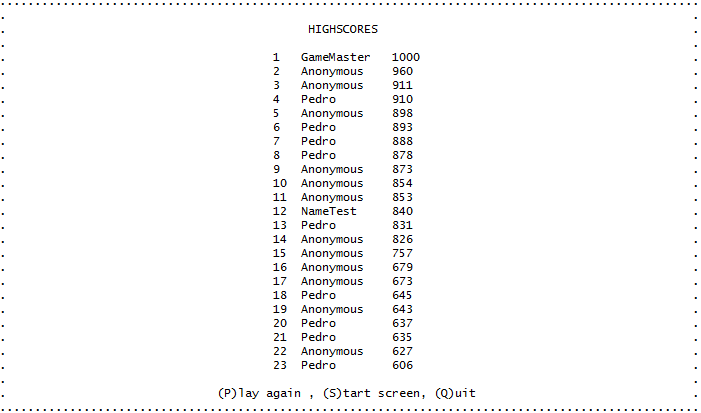
\includegraphics[width=0.6\paperwidth]{images/hscore_test_noname2}
	\caption{The score and "Anonymous" are displayed correctly and in the right order}
	\label{fig:hscore_test_noname2} 
	\end{center}
\end{figure}
\newpage
\subsubsection*{Highscore screen works with multiple screen sizes}
We've already seen the highscore table works with a screen size of 100x30.
\begin{figure}[!ht]
	\begin{center}
	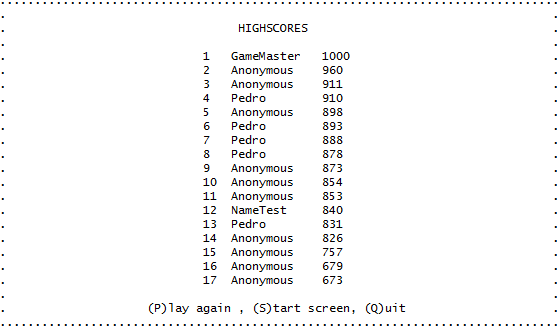
\includegraphics[width=0.6\paperwidth]{images/hscore_test_80x24}
	\caption{Screen size of 80x24}
	\label{fig:hscore_test_80x24} 
	\end{center}
\end{figure}
\begin{figure}[!ht]
	\begin{center}
	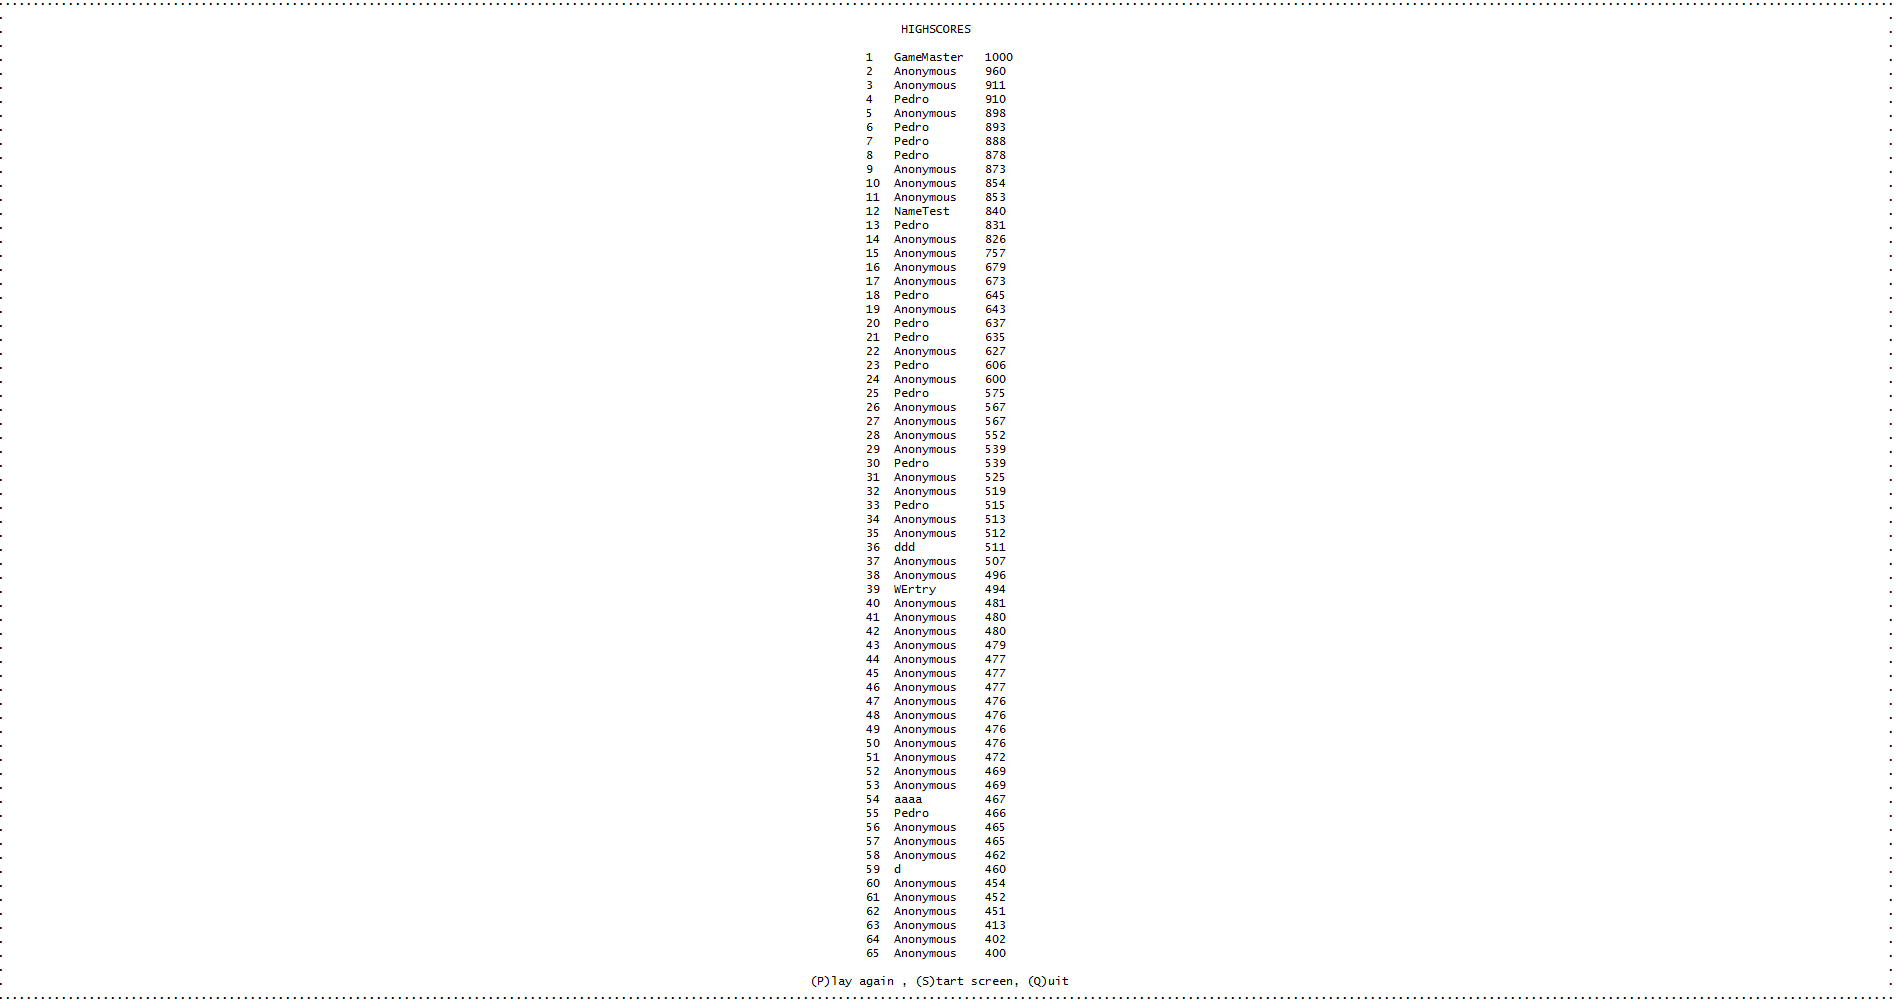
\includegraphics[width=0.6\paperwidth]{images/hscore_test_270x70}
	\caption{Screen size of 270x70}
	\label{fig:hscore_test_270x70} 
	\end{center}
\end{figure}
\newpage
\subsubsection*{File correctly represents what is shown}
This test verifies that everything is being written to the files properly and that the arrays correctly hold the data from the file.If we compare what is shown in Figure \ref{fig:hscore_test_noname2} with Figure \ref{fig:hscore_test_file}, we can see that the \emph{highscores} file correctly represents what is shown on the screen and vice versa.
\begin{figure}[!ht]
	\begin{center}
	\includegraphics[width=0.22\paperwidth]{images/hscore_test_file}
	\caption{The contents in \emph{highscores}}
	\label{fig:hscore_test_file} 
	\end{center}
\end{figure}
\clearpage
\end{document}
